\documentclass[12pt,letterpaper]{article}
\usepackage{natbib}

%Packages
\usepackage{fixltx2e}
\usepackage{textcomp}
\usepackage{fullpage}
\usepackage{float}
\usepackage{latexsym}
\usepackage{url}
\usepackage{epsfig}
\usepackage{graphicx}
\usepackage{amssymb}
\usepackage{amsmath}
\usepackage{mathtools}
\usepackage{bm}
\usepackage{array}
\usepackage[version=3]{mhchem}
\usepackage{ifthen}
\usepackage{caption}
\usepackage{hyperref}
\usepackage{amsthm}
\usepackage{amstext}
\usepackage{enumerate}
\usepackage[osf]{mathpazo}
\usepackage{dcolumn}
\usepackage{lineno}
\usepackage{pdflscape}
\usepackage{longtable}

\DeclarePairedDelimiter\abs{\lvert}{\rvert}%
\DeclarePairedDelimiter\norm{\lVert}{\rVert}%
\newcolumntype{d}[1]{D{.}{.}{#1}}

\pagenumbering{arabic}


%Pagination style and stuff
\linespread{2}
\raggedright
\setlength{\parindent}{0.5in}
\setcounter{secnumdepth}{0} 
\renewcommand{\section}[1]{%
\bigskip
\begin{center}
\begin{Large}
\normalfont\scshape #1
\medskip
\end{Large}
\end{center}}
\renewcommand{\subsection}[1]{%
\bigskip
\begin{center}
\begin{large}
\normalfont\itshape #1
\end{large}
\end{center}}
\renewcommand{\subsubsection}[1]{%
\vspace{2ex}
\noindent
\textit{#1.}---}
\renewcommand{\tableofcontents}{}
%\bibpunct{(}{)}{;}{a}{}{,}

%---------------------------------------------
%
%       START
%
%---------------------------------------------

\begin{document}

%Running head
\begin{flushright}
Version dated: \today
\end{flushright}
\bigskip
\noindent RH: Characters correlation

\bigskip
\medskip
\begin{center}
\noindent{\Large \bf Influence of different modes of morphological character correlation on phylogenetic tree inference}

\bigskip

\noindent{\Large \bf Supplementary material 3 - Additional results}

\bigskip

\noindent {\normalsize \sc Thomas Guillerme$^{1,2,*}$, and Martin D. Brazeau$^{2,3}$}\\
\noindent {\small \it 
$^1$School of Biological Sciences, University of Queensland, St. Lucia, Queensland, Australia.\\
$^2$Imperial College London, Silwood Park Campus, Department of Life Sciences, Buckhurst Road, Ascot SL5 7PY, United Kingdom.\\
$^3$Department of Earth Sciences, Natural History Museum, Cromwell Road, London, SW75BD, United Kingdom.\\}

\end{center}
\medskip
\noindent{*\bf Corresponding author.} \textit{guillert@tcd.ie}\\ 
\vspace{1in}

%Line numbering
% \modulolinenumbers[1]
% \linenumbers

\newpage

\section{Changes in average Character Difference}

The following figures and tables represent the average change in the Character difference metric for the ``maximised'', ``minimised'' and ``randomised'' matrices compared to the ``normal'' matrix.

\begin{figure}[!htbp]
\centering
   \includegraphics[width=0.75\textwidth]{../Figures/Difference_change_maxi.pdf}
\caption{Average Character Difference change in all the ``maximised'' matrices for 25, 75 and 150 taxa and 100, 350 and 1000 characters.}
\end{figure}

\begin{figure}[!htbp]
\centering
   \includegraphics[width=0.75\textwidth]{../Figures/Difference_change_mini.pdf}
\caption{Average Character Difference change in all the ``minimised'' matrices for 25, 75 and 150 taxa and 100, 350 and 1000 characters.}
\end{figure}

\begin{figure}[!htbp]
\centering
   \includegraphics[width=0.75\textwidth]{../Figures/Difference_change_rand.pdf}
\caption{Average Character Difference change in all the ``randomised'' matrices for 25, 75 and 150 taxa and 100, 350 and 1000 characters.}
\end{figure}


% latex table generated in R 4.1.3 by xtable 1.8-4 package
% Thu Mar 24 13:38:33 2022
\begin{table}[ht]
\centering
\begin{tabular}{rrll}
  \hline
 & statistic & p.value & bhatt.coeff \\ 
  \hline
maxi - mini & 32396.000 & \textbf{0} & \textbf{0.049} \\ 
  maxi - rand & 31203.000 & \textbf{0} & 0.415 \\ 
  mini - rand & 662.000 & \textbf{0} & 0.307 \\ 
  150t - 25t & 17046.000 & 1 & 0.938 \\ 
  150t - 75t & 16067.000 & 1 & \textbf{0.959} \\ 
  25t - 75t & 15161.000 & 0.879 & 0.926 \\ 
  1000c - 100c & 16500.000 & 1 & 0.947 \\ 
  1000c - 350c & 15539.000 & 1 & \textbf{0.956} \\ 
  100c - 350c & 15330.000 & 1 & \textbf{0.973} \\ 
   \hline
\end{tabular}
\caption{Pairwise Wilcoxon test and Bhattacharrya Coefficients for the differences incharacter difference for the different scenarios, number of taxa and characters.} 
\label{Tab_difference_change}
\end{table}


\newpage

\section{Proportions of duplicated characters}

The following figures and tables represent the proportions duplicated characters for the ``maximised'', ``minimised'' and ``randomised'' matrices compared to the ``normal'' matrix. This represents the amount of character modified in the matrices. In other words, when modifying the matrices, a character can be removed a replace by either a character already present in the matrix (duplicated character) or by a character removed (replaced character).

\begin{figure}[!htbp]
\centering
   \includegraphics[width=0.75\textwidth]{../Figures/Proportion_duplicated_maxi.pdf}
\caption{Proportion of duplicated characters in all the ``maximised'' matrices for 25, 75 and 150 taxa and 100, 350 and 1000 characters.}
\end{figure}

\begin{figure}[!htbp]
\centering
   \includegraphics[width=0.75\textwidth]{../Figures/Proportion_duplicated_mini.pdf}
\caption{Proportion of duplicated characters in all the ``minimised'' matrices for 25, 75 and 150 taxa and 100, 350 and 1000 characters.}
\end{figure}

\begin{figure}[!htbp]
\centering
   \includegraphics[width=0.75\textwidth]{../Figures/Proportion_duplicated_rand.pdf}
\caption{Proportion of duplicated characters in all the ``randomised'' matrices for 25, 75 and 150 taxa and 100, 350 and 1000 characters.}
\end{figure}


% latex table generated in R 4.1.3 by xtable 1.8-4 package
% Thu Mar 24 13:38:33 2022
\begin{table}[ht]
\centering
\begin{tabular}{rrll}
  \hline
 & statistic & p.value & bhatt.coeff \\ 
  \hline
maxi - mini & 29735.500 & \textbf{0} & 0.363 \\ 
  maxi - rand & 6546.500 & \textbf{0} & 0.553 \\ 
  mini - rand & 2685.500 & \textbf{0} & 0.366 \\ 
  150t - 25t & 12742.000 & \textbf{0.001} & 0.935 \\ 
  150t - 75t & 14725.000 & 0.406 & \textbf{0.977} \\ 
  25t - 75t & 18284.000 & 0.104 & 0.909 \\ 
  1000c - 100c & 14982.500 & 0.653 & \textbf{0.973} \\ 
  1000c - 350c & 16059.500 & 1 & \textbf{0.984} \\ 
  100c - 350c & 17210.500 & 0.919 & \textbf{0.974} \\ 
   \hline
\end{tabular}
\caption{Pairwise Wilcoxon test and Bhattacharrya Coefficients for the difference in proportion of character duplicated for the different scenarios, number of taxa and characters.} 
\label{Tab_proportion_duplicated}
\end{table}



\newpage

\section{Signal to noise ratio}

\begin{figure}[!htbp]
\centering
   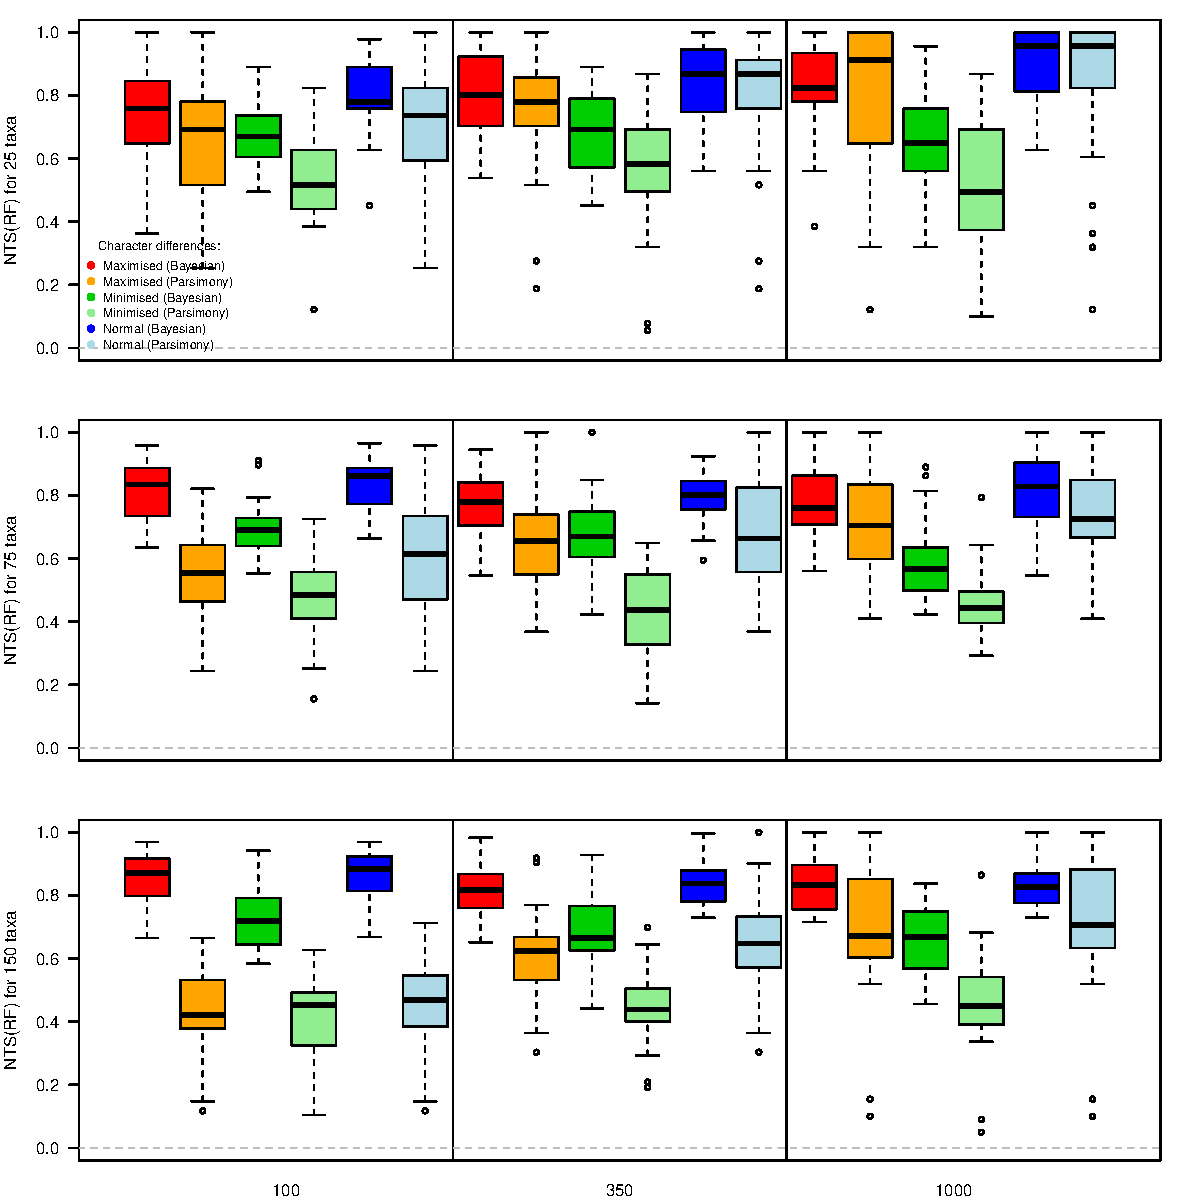
\includegraphics[width=1\textwidth]{../Figures/RF_results_null.pdf} 
\caption{\small{Effect of Character Difference on recovering the ``random'' topology. The y axis represents the Normalised Tree Similarity using Robinson-Fould distance for matrices with 25, 75 and 150 taxa from top to bottom respectively. The x axis represents the different Character Difference scenarios and tree inference method with the Maximised Character Difference in Bayesian (red) and under Maximum Parsimony (orange), the Minimised Character Difference in Bayesian (dark green) and under Maximum Parsimony (light green) and the Randomised Character Difference in Bayesian (dark blue) and under Maximum Parsimony (light blue) for matrices of 100, 350 and 1000 characters in the panels from left to right.}}
\label{Fig:RF_results_rand}
\end{figure}


\begin{figure}[!htbp]
\centering
   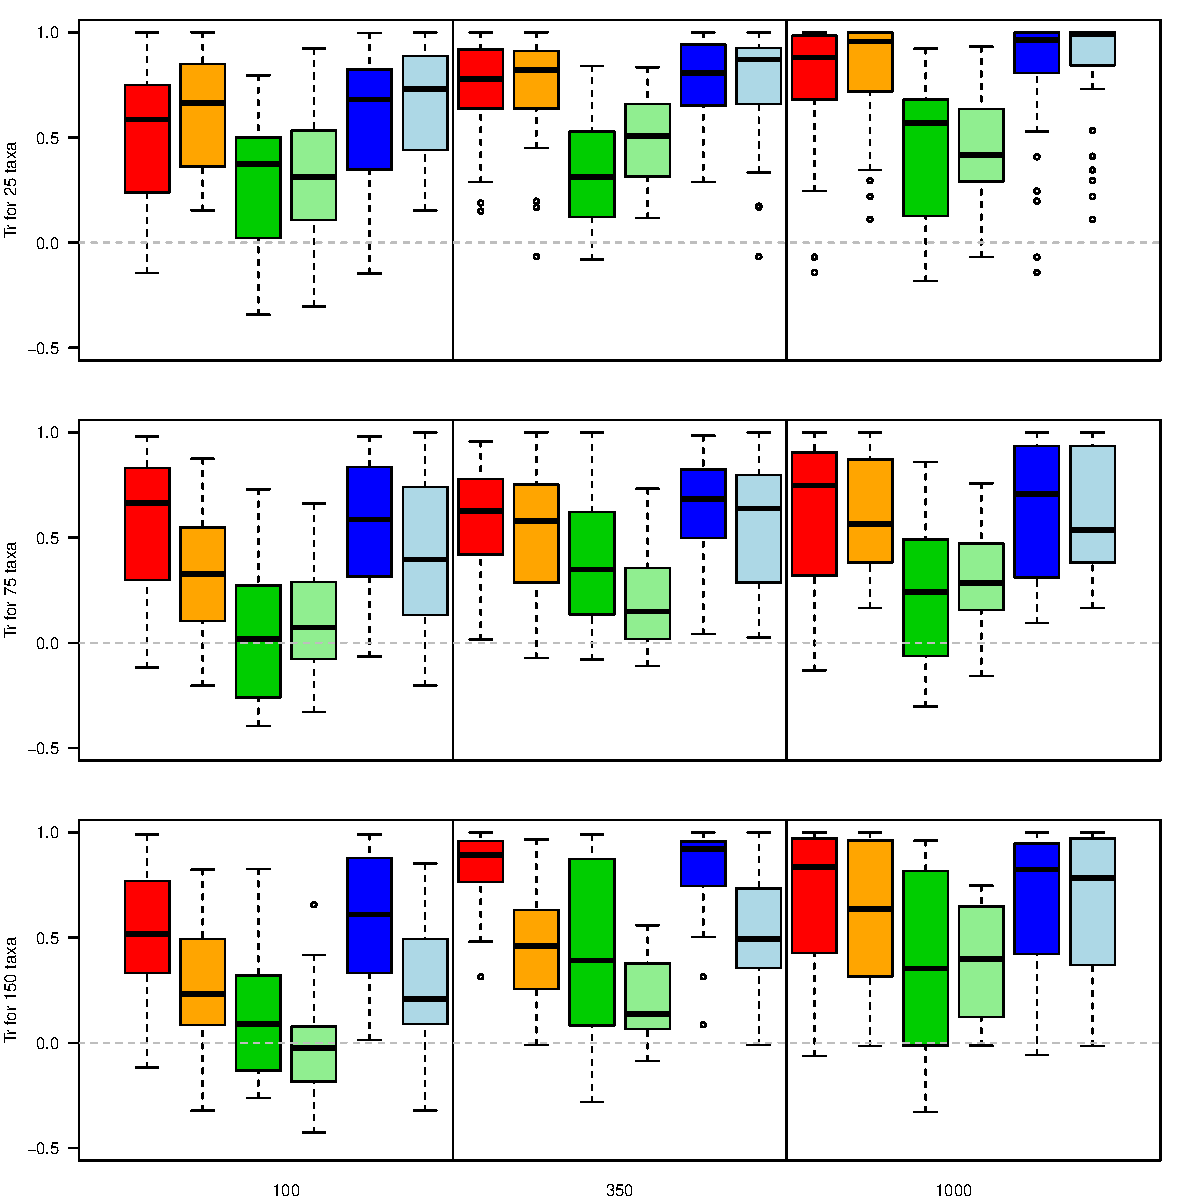
\includegraphics[width=1\textwidth]{../Figures/Tr_results_null.pdf}
\caption{Effect of Character Difference on recovering the ``random'' topology. The axis are identical to figure \ref{Fig:RF_results_rand} but y axis represents the Normalised Tree Similarity using Triplets distance.}
\label{Fig:Tr_results_rand}
\end{figure}

\newpage

\section{Tree resolution}

\begin{figure}[!htbp]
\centering
   \includegraphics[width=1\textwidth]{../Figures/Resolution_25t.pdf}
\caption{Node resolution for the trees with 25 taxa. The y axis represents the number of nodes in the tree. The horizontal lines are the distributions of resolved nodes per trees per number of characters (100c, 350c and 1000c), per matrix type (normal: norm, maxi: maximised, mini: minimised, rand: randomised - respectively in grey, red, green and blue) and per method (bay: Bayesian and par: maximum parsimony - respectively in dark and light colours). The black dots, thick solid lines and dashed lines represent respectively the median, 50\% CI and 95\% CI of the distribution.}
\label{Fig:Resolution_25t}
\end{figure}

\begin{figure}[!htbp]
\centering
   \includegraphics[width=1\textwidth]{../Figures/Resolution_75t.pdf}
\caption{Node resolution for the trees with 75 taxa. The y axis represents the number of nodes in the tree. The horizontal lines are the distributions of resolved nodes per trees per number of characters (100c, 350c and 1000c), per matrix type (normal: norm, maxi: maximised, mini: minimised, rand: randomised - respectively in grey, red, green and blue) and per method (bay: Bayesian and par: maximum parsimony - respectively in dark and light colours). The black dots, thick solid lines and dashed lines represent respectively the median, 50\% CI and 95\% CI of the distribution.}
\label{Fig:Resolution_75t}
\end{figure}

\begin{figure}[!htbp]
\centering
   \includegraphics[width=1\textwidth]{../Figures/Resolution_150t.pdf}
\caption{Node resolution for the trees with 150 taxa. The y axis represents the number of nodes in the tree. The horizontal lines are the distributions of resolved nodes per trees per number of characters (100c, 350c and 1000c), per matrix type (normal: norm, maxi: maximised, mini: minimised, rand: randomised - respectively in grey, red, green and blue) and per method (bay: Bayesian and par: maximum parsimony - respectively in dark and light colours). The black dots, thick solid lines and dashed lines represent respectively the median, 50\% CI and 95\% CI of the distribution.}
\label{Fig:Resolution_150t}
\end{figure}

\newpage

\section{Ability to recover the ``true'' tree}


\begin{figure}[!htbp]
\centering
   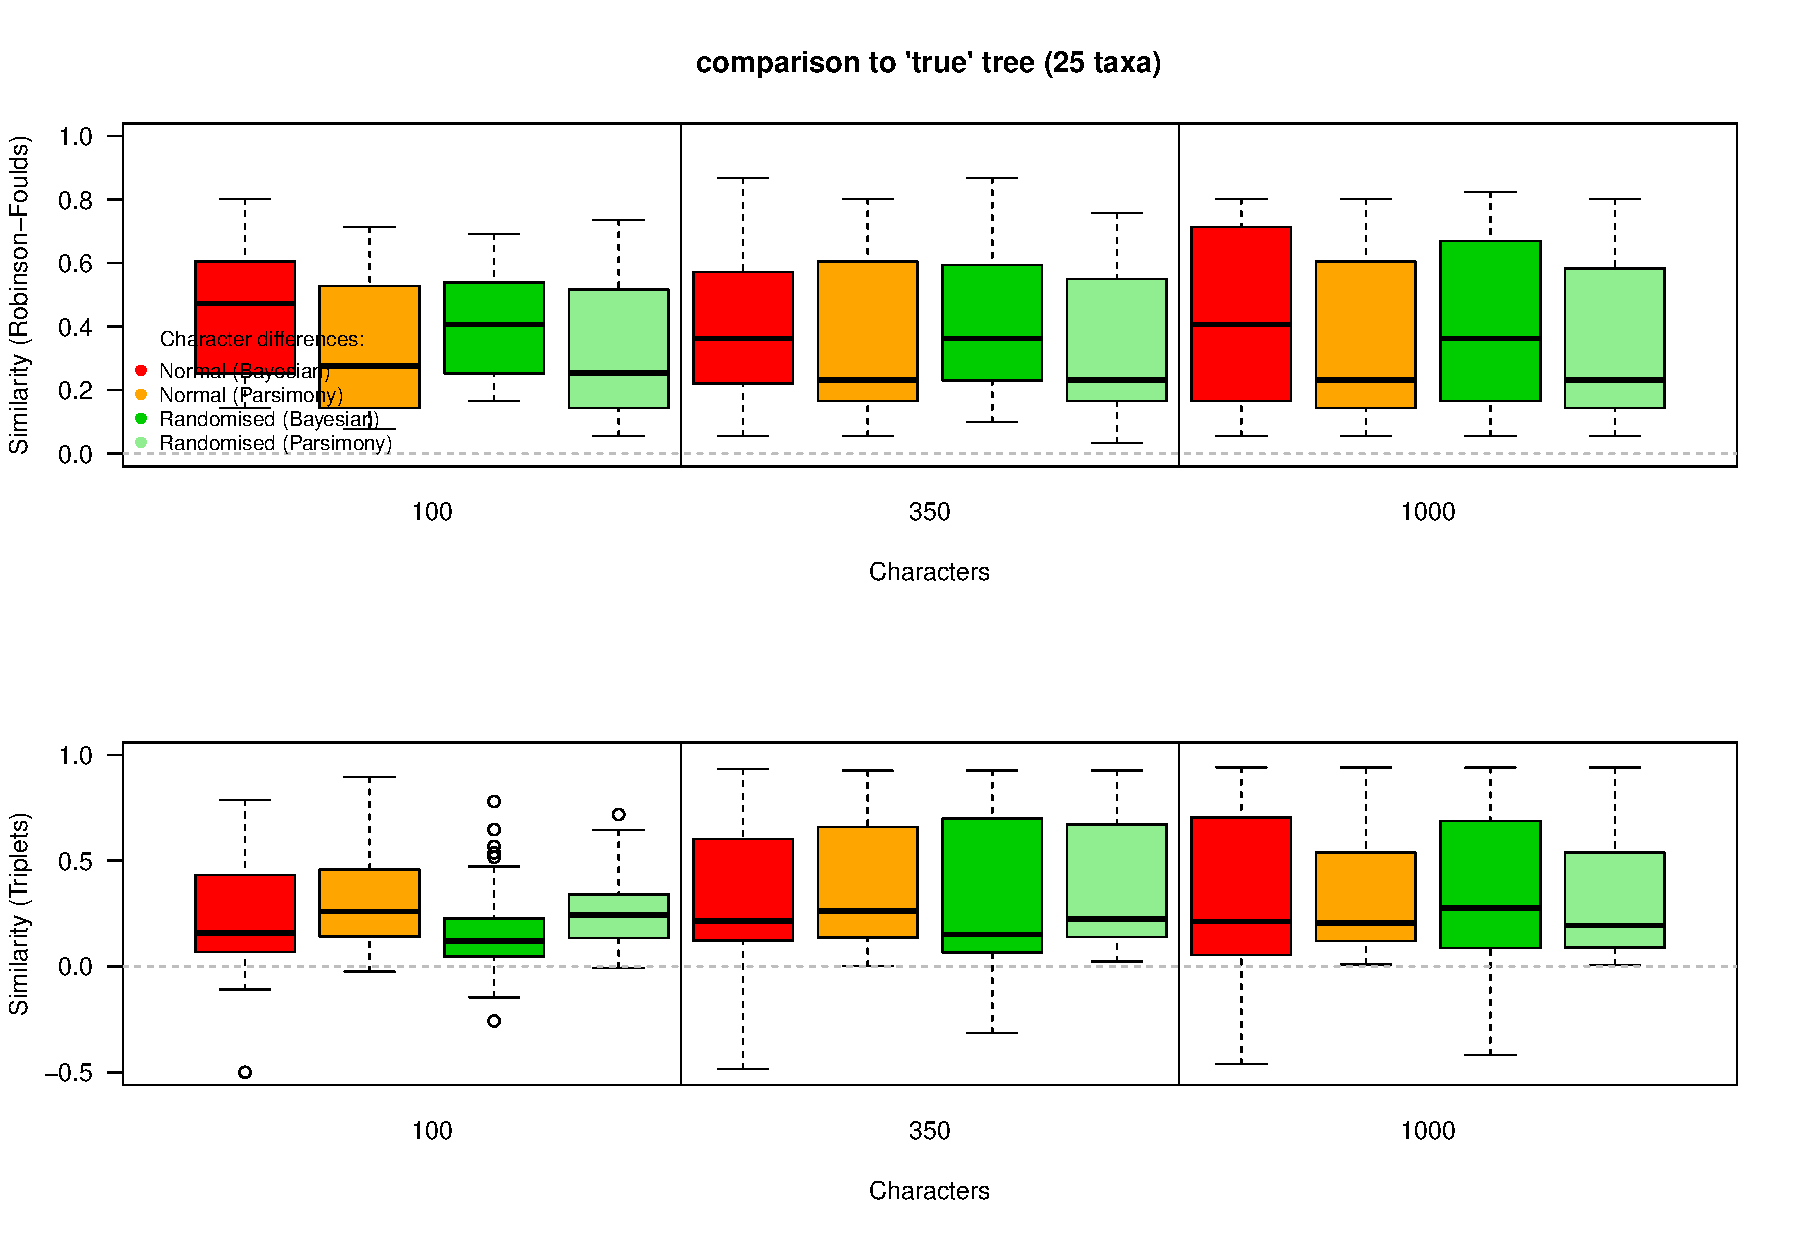
\includegraphics[width=1\textwidth]{../Figures/25t_true_tree.pdf}
\caption{Ability to recover the ``true'' tree for the ``normal'' matrix (in red or orange) and for the ``randomised'' matrix for 25 taxa using Bayesian inference (dark colours) or maximum parsimony (light colours) measured in terms of clade conservation ($NTS_{RF}$, upper panel) and taxa displacement ($NTS_{Tr}$, lower panel).}
\end{figure}

\begin{figure}[!htbp]
\centering
   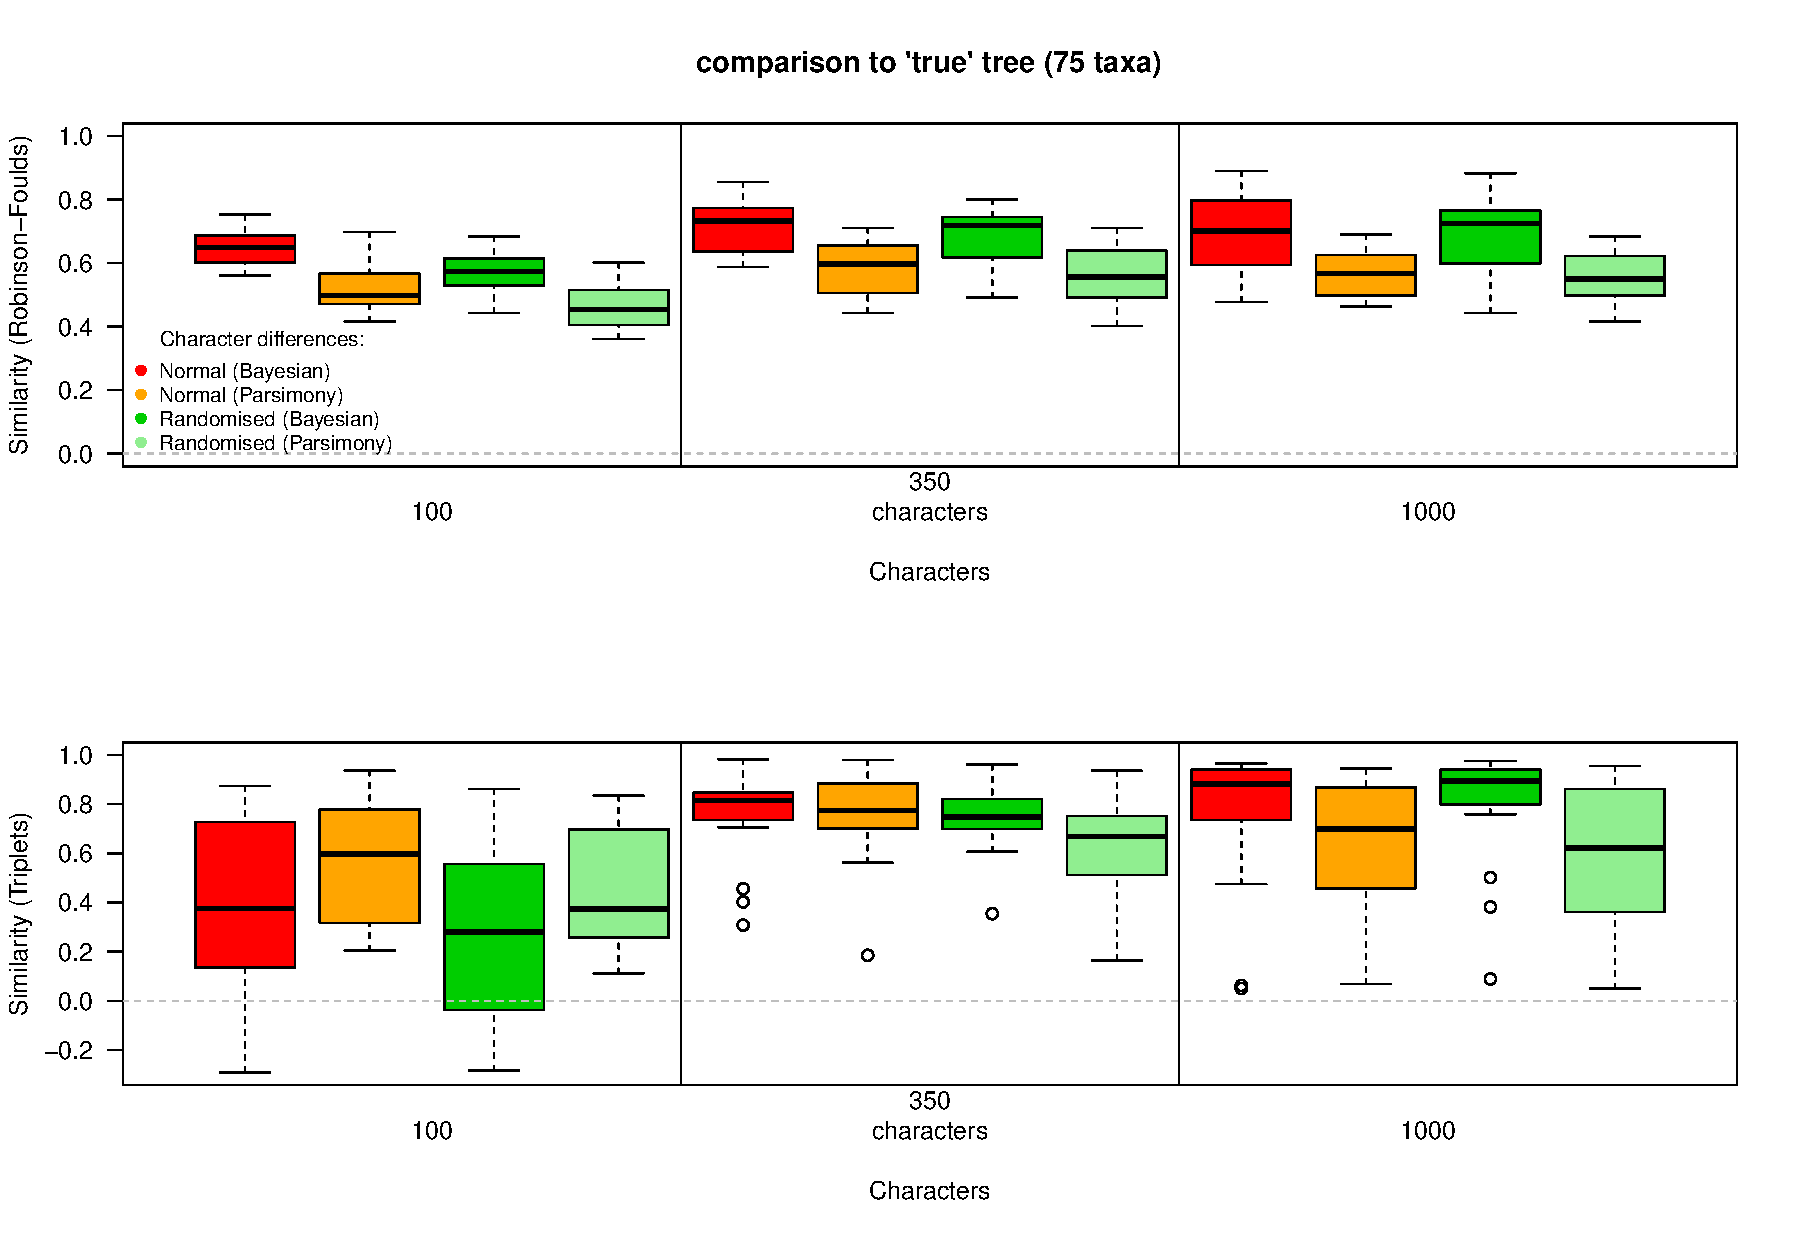
\includegraphics[width=1\textwidth]{../Figures/75t_true_tree.pdf}
\caption{Ability to recover the ``true'' tree for the ``normal'' matrix (in red or orange) and for the ``randomised'' matrix for 75 taxa using Bayesian inference (dark colours) or maximum parsimony (light colours) measured in terms of clade conservation ($NTS_{RF}$, upper panel) and taxa displacement ($NTS_{Tr}$, lower panel).}
\end{figure}

\begin{figure}[!htbp]
\centering
   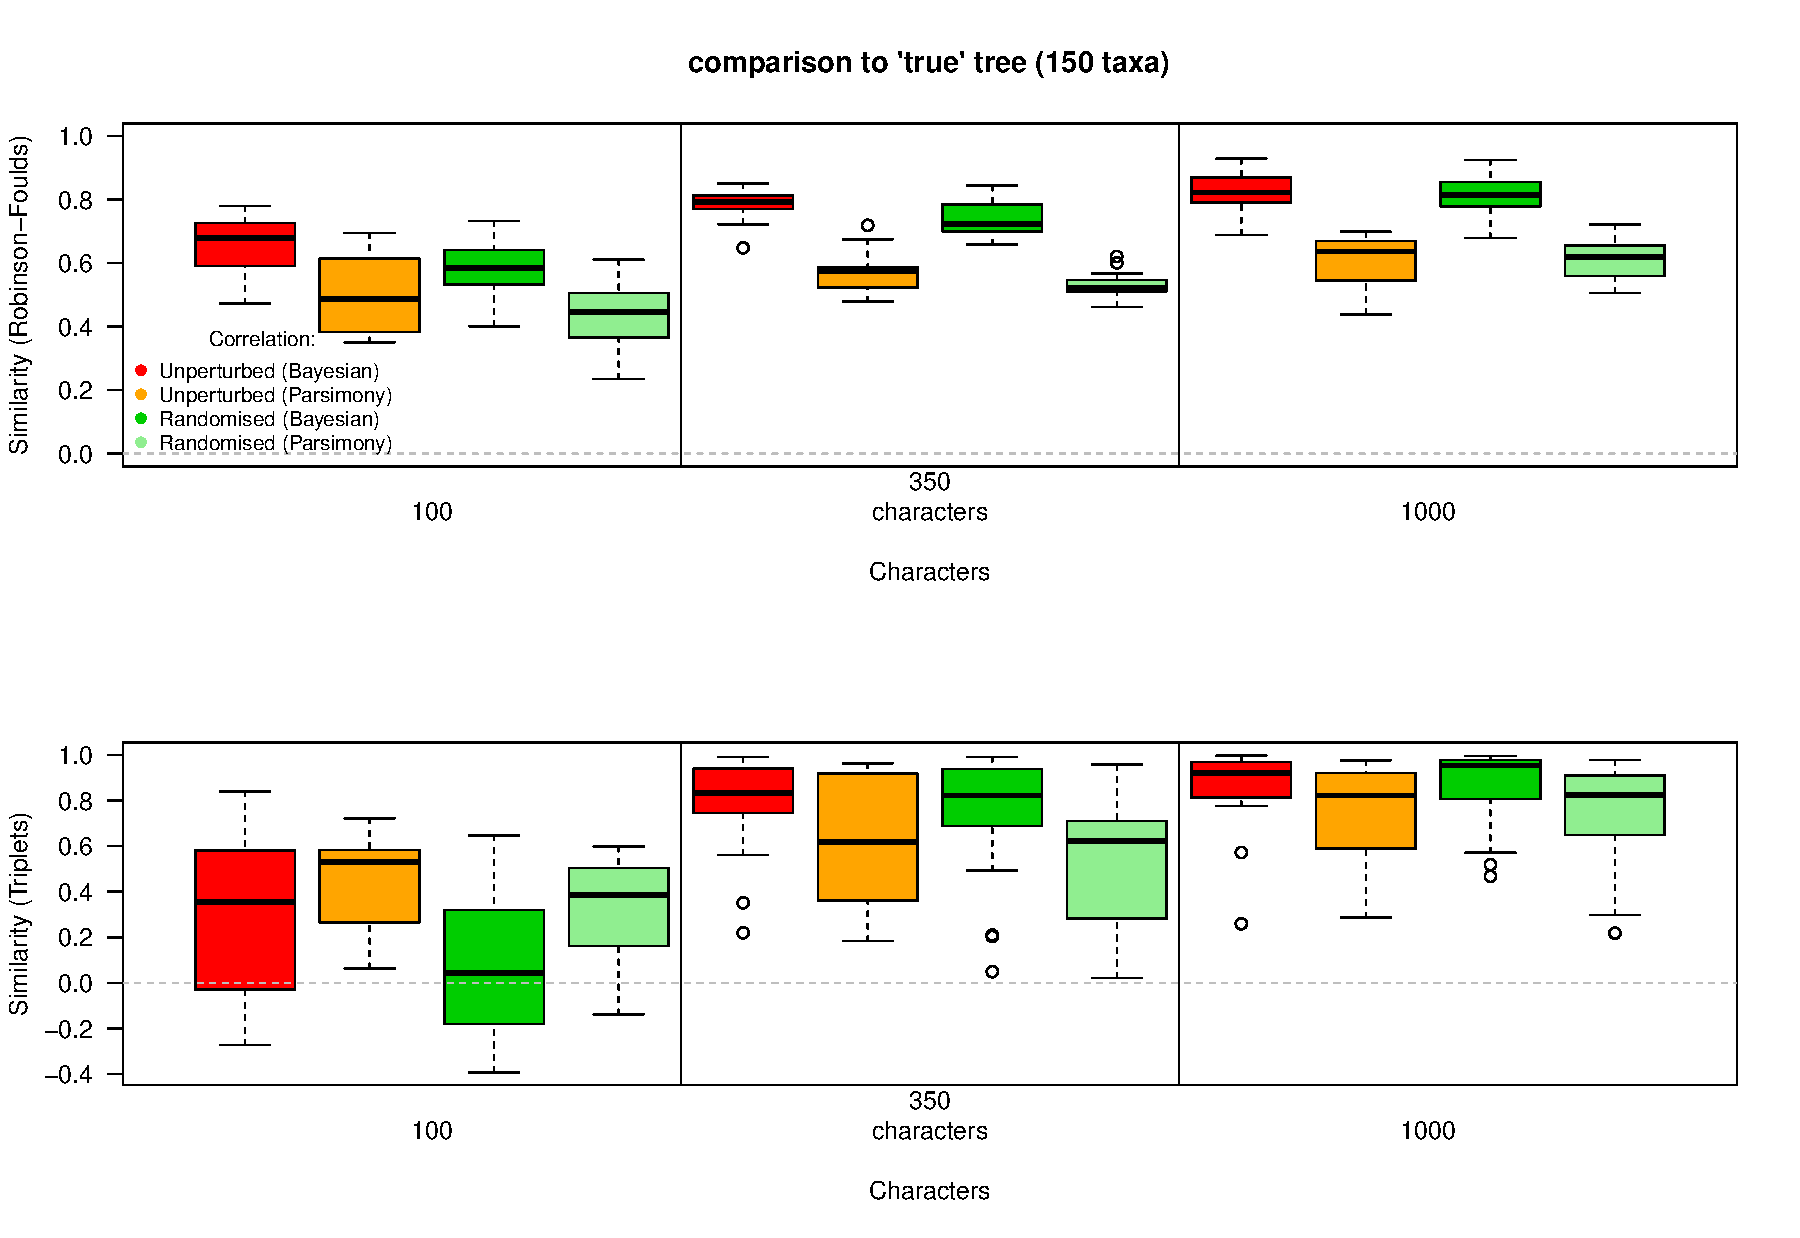
\includegraphics[width=1\textwidth]{../Figures/150t_true_tree.pdf}
\caption{Ability to recover the ``true'' tree for the ``normal'' matrix (in red or orange) and for the ``randomised'' matrix for 150 taxa using Bayesian inference (dark colours) or maximum parsimony (light colours) measured in terms of clade conservation ($NTS_{RF}$, upper panel) and taxa displacement ($NTS_{Tr}$, lower panel).}
\end{figure}


\newpage

\section{Pooled results distributions}

% latex table generated in R 3.4.4 by xtable 1.8-2 package
% Tue Mar 27 15:27:13 2018
\begin{table}[ht]
\centering
\begin{tabular}{lllrrrrrr}
  \hline
comp & metric & scenario & Min. & 1st Qu. & Median & Mean & 3rd Qu. & Max. \\ 
  \hline
Best & RF & maxi & 0.407 & 0.802 & 0.956 & 0.885 & 1.000 & 1.000 \\ 
   &  & mini & 0.076 & 0.471 & 0.605 & 0.594 & 0.726 & 0.956 \\ 
   &  & rand & 0.100 & 0.656 & 0.792 & 0.762 & 0.894 & 1.000 \\ 
   & Tr & maxi & -0.031 & 0.749 & 0.964 & 0.839 & 1.000 & 1.000 \\ 
   &  & mini & -0.473 & 0.050 & 0.303 & 0.312 & 0.592 & 0.980 \\ 
   &  & rand & -0.323 & 0.370 & 0.713 & 0.628 & 0.926 & 1.000 \\ 
  Null & RF & maxi & 0.100 & 0.619 & 0.758 & 0.731 & 0.868 & 1.000 \\ 
   &  & mini & 0.049 & 0.457 & 0.584 & 0.574 & 0.705 & 1.000 \\ 
   &  & norm & 0.100 & 0.656 & 0.792 & 0.762 & 0.894 & 1.000 \\ 
   & Tr & maxi & -0.323 & 0.338 & 0.651 & 0.597 & 0.889 & 1.000 \\ 
   &  & mini & -0.427 & 0.027 & 0.276 & 0.284 & 0.535 & 1.000 \\ 
   &  & norm & -0.323 & 0.370 & 0.713 & 0.628 & 0.926 & 1.000 \\ 
   \hline
\end{tabular}
\caption{Summary statistics of the normalised distances to the best or null tree for the pooled scenarios.} 
\label{Full_Tab_pooledscenarios}
\end{table}


\newpage

% latex table generated in R 3.4.4 by xtable 1.8-2 package
% Tue Mar 27 15:27:15 2018
\begin{table}[ht]
\centering
\begin{tabular}{lllrrrrrr}
  \hline
comp & metric & character & Min. & 1st Qu. & Median & Mean & 3rd Qu. & Max. \\ 
  \hline
Best & RF & c100 & 0.107 & 0.583 & 0.758 & 0.730 & 0.892 & 1.000 \\ 
   &  & c350 & 0.077 & 0.623 & 0.773 & 0.745 & 0.912 & 1.000 \\ 
   &  & c1000 & 0.076 & 0.615 & 0.821 & 0.767 & 0.971 & 1.000 \\ 
   & Tr & c100 & -0.473 & 0.161 & 0.544 & 0.497 & 0.863 & 1.000 \\ 
   &  & c350 & -0.307 & 0.363 & 0.693 & 0.622 & 0.936 & 1.000 \\ 
   &  & c1000 & -0.276 & 0.372 & 0.799 & 0.659 & 0.992 & 1.000 \\ 
  Null & RF & c100 & 0.103 & 0.517 & 0.670 & 0.658 & 0.814 & 1.000 \\ 
   &  & c350 & 0.055 & 0.583 & 0.718 & 0.694 & 0.824 & 1.000 \\ 
   &  & c1000 & 0.049 & 0.576 & 0.739 & 0.715 & 0.871 & 1.000 \\ 
   & Tr & c100 & -0.427 & 0.076 & 0.368 & 0.375 & 0.677 & 1.000 \\ 
   &  & c350 & -0.282 & 0.295 & 0.603 & 0.551 & 0.839 & 1.000 \\ 
   &  & c1000 & -0.328 & 0.295 & 0.620 & 0.582 & 0.930 & 1.000 \\ 
   \hline
\end{tabular}
\caption{Summary statistics of the normalised distances to the best or null tree for the pooled number of characters.} 
\label{Full_Tab_pooledcharacters}
\end{table}


\newpage

% latex table generated in R 3.4.4 by xtable 1.8-2 package
% Tue Mar 27 15:27:15 2018
\begin{table}[ht]
\centering
\begin{tabular}{lllrrrrrr}
  \hline
comp & metric & taxa & Min. & 1st Qu. & Median & Mean & 3rd Qu. & Max. \\ 
  \hline
Best & RF & t25 & 0.077 & 0.648 & 0.802 & 0.772 & 0.934 & 1.000 \\ 
   &  & t75 & 0.155 & 0.595 & 0.760 & 0.737 & 0.904 & 1.000 \\ 
   &  & t150 & 0.076 & 0.578 & 0.763 & 0.732 & 0.915 & 1.000 \\ 
   & Tr & t25 & -0.436 & 0.463 & 0.758 & 0.670 & 0.964 & 1.000 \\ 
   &  & t75 & -0.473 & 0.237 & 0.588 & 0.543 & 0.920 & 1.000 \\ 
   &  & t150 & -0.424 & 0.238 & 0.615 & 0.565 & 0.955 & 1.000 \\ 
  Null & RF & t25 & 0.055 & 0.605 & 0.758 & 0.729 & 0.890 & 1.000 \\ 
   &  & t75 & 0.141 & 0.548 & 0.691 & 0.672 & 0.814 & 1.000 \\ 
   &  & t150 & 0.049 & 0.533 & 0.689 & 0.667 & 0.827 & 1.000 \\ 
   & Tr & t25 & -0.343 & 0.370 & 0.665 & 0.606 & 0.902 & 1.000 \\ 
   &  & t75 & -0.395 & 0.184 & 0.429 & 0.435 & 0.739 & 1.000 \\ 
   &  & t150 & -0.427 & 0.137 & 0.472 & 0.467 & 0.826 & 1.000 \\ 
   \hline
\end{tabular}
\caption{Summary statistics of the normalised distances to the best or null tree for the pooled number of taxa.} 
\label{Full_Tab_pooledtaxa}
\end{table}


\newpage

% latex table generated in R 3.4.4 by xtable 1.8-2 package
% Tue Mar 27 15:27:15 2018
\begin{table}[ht]
\centering
\begin{tabular}{lllrrrrrr}
  \hline
comp & metric & method & Min. & 1st Qu. & Median & Mean & 3rd Qu. & Max. \\ 
  \hline
Best & RF & bayesian & 0.319 & 0.714 & 0.828 & 0.811 & 0.934 & 1.000 \\ 
   &  & parsimony & 0.076 & 0.496 & 0.679 & 0.684 & 0.911 & 1.000 \\ 
   & Tr & bayesian & -0.473 & 0.354 & 0.738 & 0.618 & 0.947 & 1.000 \\ 
   &  & parsimony & -0.436 & 0.258 & 0.601 & 0.568 & 0.949 & 1.000 \\ 
  Null & RF & bayesian & 0.319 & 0.684 & 0.780 & 0.770 & 0.871 & 1.000 \\ 
   &  & parsimony & 0.049 & 0.457 & 0.601 & 0.608 & 0.758 & 1.000 \\ 
   & Tr & bayesian & -0.395 & 0.276 & 0.608 & 0.538 & 0.856 & 1.000 \\ 
   &  & parsimony & -0.427 & 0.194 & 0.468 & 0.468 & 0.750 & 1.000 \\ 
   \hline
\end{tabular}
\caption{Summary statistics of the normalised distances to the best or null tree for the pooled methods.} 
\label{Full_Tab_pooledmethod}
\end{table}


\newpage

\section{Pooled tests results}

% latex table generated in R 3.5.3 by xtable 1.8-3 package
% Tue Apr 16 16:10:49 2019
\begin{table}[ht]
\centering
\begin{tabular}{lllrrr}
  \hline
comp & metric & test & bhatt.coeff & statistic & p.value \\ 
  \hline
Best & RF & maxi:mini & 0.848 & 32012.500 & 0.000 \\ 
   &  & maxi:rand & 0.941 & 44161.000 & 0.000 \\ 
   &  & mini:rand & 0.954 & 80382.500 & 0.000 \\ 
   & Tr & maxi:mini & 0.992 & 60680.500 & 1.000 \\ 
   &  & maxi:rand & 0.980 & 60447.000 & 1.000 \\ 
   &  & mini:rand & 0.982 & 64222.500 & 1.000 \\ 
  Null & RF & maxi:mini & 0.938 & 44768.000 & 0.000 \\ 
   &  & maxi:norm & 0.902 & 35764.500 & 0.000 \\ 
   &  & mini:norm & 0.978 & 53007.000 & 0.000 \\ 
   & Tr & maxi:mini & 0.985 & 63723.000 & 1.000 \\ 
   &  & maxi:norm & 0.966 & 51652.500 & 0.000 \\ 
   &  & mini:norm & 0.965 & 52882.000 & 0.000 \\ 
   \hline
\end{tabular}
\caption{Difference between the pooled scenarios. Bhatt.coeff is the Bhattacharrya Coefficient (probability of overlap), the statistic and the p.value are from a non-parametric wilcoxon test (with Bonferonni-Holm correciton)} 
\label{Full_Tab_pooledscenarios_test}
\end{table}


\newpage

% latex table generated in R 4.1.3 by xtable 1.8-4 package
% Thu Mar 24 14:25:28 2022
\begin{table}[ht]
\centering
\begin{tabular}{lllrrr}
  \hline
comp & metric & test & bhatt.coeff & statistic & p.value \\ 
  \hline
Best & RF & c100 vs. c350 & 0.965 & 48263.500 & 0.000 \\ 
   &  & c100 vs. c1000 & 0.914 & 37714.500 & 0.000 \\ 
   &  & c350 vs. c1000 & 0.976 & 53138.000 & 0.000 \\ 
   & Tr & c100 vs. c350 & 0.929 & 40253.000 & 0.000 \\ 
   &  & c100 vs. c1000 & 0.826 & 27923.000 & 0.000 \\ 
   &  & c350 vs. c1000 & 0.957 & 48164.500 & 0.000 \\ 
  Null & RF & c100 vs. c350 & 0.930 & 44273.000 & 0.000 \\ 
   &  & c100 vs. c1000 & 0.847 & 31820.000 & 0.000 \\ 
   &  & c350 vs. c1000 & 0.961 & 50112.500 & 0.000 \\ 
   & Tr & c100 vs. c350 & 0.923 & 39035.000 & 0.000 \\ 
   &  & c100 vs. c1000 & 0.804 & 24621.500 & 0.000 \\ 
   &  & c350 vs. c1000 & 0.935 & 45220.000 & 0.000 \\ 
   \hline
\end{tabular}
\caption{Difference between the pooled number of characters. Bhatt.coeff is the Bhattacharrya Coefficient (probability of overlap), the statistic and the p.value are from a non-parametric wilcoxon test (with Bonferonni-Holm correciton)} 
\label{Full_Tab_pooledscharacters_test}
\end{table}


\newpage

% latex table generated in R 3.4.4 by xtable 1.8-2 package
% Tue Mar 27 13:20:37 2018
\begin{table}[ht]
\centering
\begin{tabular}{lllrrr}
  \hline
comp & metric & test & bhatt.coeff & statistic & p.value \\ 
  \hline
Best & RF & t25:t75 & 0.976 & 218421.000 & 0.023 \\ 
   &  & t25:t150 & 0.988 & 220529.000 & 0.007 \\ 
   &  & t75:t150 & 0.990 & 201037.000 & 1.000 \\ 
   & Tr & t25:t75 & 0.976 & 233282.000 & 0.000 \\ 
   &  & t25:t150 & 0.978 & 227288.000 & 0.000 \\ 
   &  & t75:t150 & 0.992 & 194201.000 & 1.000 \\ 
  Null & RF & t25:t75 & 0.959 & 237247.000 & 0.000 \\ 
   &  & t25:t150 & 0.978 & 234937.000 & 0.000 \\ 
   &  & t75:t150 & 0.983 & 196946.000 & 1.000 \\ 
   & Tr & t25:t75 & 0.961 & 255239.000 & 0.000 \\ 
   &  & t25:t150 & 0.969 & 242327.000 & 0.000 \\ 
   &  & t75:t150 & 0.986 & 188297.000 & 1.000 \\ 
   \hline
\end{tabular}
\caption{Difference between the pooled number of taxa. Bhatt.coeff is the Bhattacharrya Coefficient (probability of overlap), the statistic and the p.value are from a non-parametric wilcoxon test (with Bonferonni-Holm correciton)} 
\label{Full_Tab_pooledstaxa_test}
\end{table}


\newpage

% latex table generated in R 3.5.3 by xtable 1.8-3 package
% Tue Apr 23 11:45:02 2019
\begin{table}[ht]
\centering
\begin{tabular}{lllrrr}
  \hline
comp & metric & test & bhatt.coeff & statistic & p.value \\ 
  \hline
Best & RF & bayesian:parsimony & 0.939 & 192659.000 & 0.000 \\ 
   & Tr & bayesian:parsimony & 0.986 & 157677.500 & 0.082 \\ 
  Null & RF & bayesian:parsimony & 0.944 & 193142.000 & 0.000 \\ 
   & Tr & bayesian:parsimony & 0.975 & 161621.000 & 0.008 \\ 
   \hline
\end{tabular}
\caption{Difference between the pooled methods. Bhatt.coeff is the Bhattacharrya Coefficient (probability of overlap), the statistic and the p.value are from a non-parametric wilcoxon test (with Bonferonni-Holm correciton)} 
\label{Full_Tab_pooledsmethods_test}
\end{table}


\newpage

\section{Combined results distributions}

% latex table generated in R 3.4.4 by xtable 1.8-2 package
% Tue Mar 27 15:27:16 2018
\begin{longtable}{llllrrrrrr}
  \hline
method & taxa & characters & scenario & Min. & 1st Qu. & Median & Mean & 3rd Qu. & Max. \\ 
  \hline
bayesian & 25 & 100 & maxi & 0.561 & 0.780 & 0.868 & 0.862 & 0.956 & 1.000 \\ 
   &  &  & mini & 0.451 & 0.659 & 0.714 & 0.722 & 0.813 & 0.868 \\ 
   &  &  & rand & 0.451 & 0.758 & 0.780 & 0.804 & 0.890 & 0.978 \\ 
   &  & 350 & maxi & 0.539 & 0.692 & 0.890 & 0.834 & 0.967 & 1.000 \\ 
   &  &  & mini & 0.407 & 0.561 & 0.736 & 0.692 & 0.791 & 0.934 \\ 
   &  &  & rand & 0.561 & 0.747 & 0.868 & 0.832 & 0.945 & 1.000 \\ 
   &  & 1000 & maxi & 0.407 & 0.868 & 0.934 & 0.896 & 1.000 & 1.000 \\ 
   &  &  & mini & 0.319 & 0.561 & 0.692 & 0.675 & 0.769 & 0.956 \\ 
   &  &  & rand & 0.627 & 0.813 & 0.956 & 0.901 & 1.000 & 1.000 \\ 
   & 75 & 100 & maxi & 0.650 & 0.849 & 0.986 & 0.919 & 0.993 & 1.000 \\ 
   &  &  & mini & 0.553 & 0.646 & 0.718 & 0.720 & 0.777 & 0.938 \\ 
   &  &  & rand & 0.663 & 0.773 & 0.863 & 0.843 & 0.887 & 0.966 \\ 
   &  & 350 & maxi & 0.574 & 0.863 & 0.945 & 0.905 & 0.990 & 1.000 \\ 
   &  &  & mini & 0.402 & 0.615 & 0.698 & 0.677 & 0.766 & 0.856 \\ 
   &  &  & rand & 0.595 & 0.756 & 0.801 & 0.796 & 0.845 & 0.924 \\ 
   &  & 1000 & maxi & 0.574 & 0.825 & 0.904 & 0.900 & 0.986 & 1.000 \\ 
   &  &  & mini & 0.430 & 0.502 & 0.581 & 0.607 & 0.670 & 0.945 \\ 
   &  &  & rand & 0.546 & 0.732 & 0.828 & 0.816 & 0.904 & 1.000 \\ 
   & 150 & 100 & maxi & 0.756 & 0.958 & 0.993 & 0.959 & 0.997 & 1.000 \\ 
   &  &  & mini & 0.594 & 0.674 & 0.750 & 0.756 & 0.831 & 0.942 \\ 
   &  &  & rand & 0.668 & 0.814 & 0.885 & 0.860 & 0.924 & 0.970 \\ 
   &  & 350 & maxi & 0.672 & 0.922 & 0.976 & 0.940 & 0.990 & 1.000 \\ 
   &  &  & mini & 0.459 & 0.631 & 0.679 & 0.697 & 0.775 & 0.915 \\ 
   &  &  & rand & 0.729 & 0.782 & 0.838 & 0.834 & 0.880 & 0.997 \\ 
   &  & 1000 & maxi & 0.780 & 0.883 & 0.973 & 0.933 & 0.992 & 0.997 \\ 
   &  &  & mini & 0.455 & 0.580 & 0.662 & 0.677 & 0.800 & 0.919 \\ 
   &  &  & rand & 0.729 & 0.777 & 0.827 & 0.832 & 0.870 & 1.000 \\ 
  parsimony & 25 & 100 & maxi & 0.517 & 0.725 & 0.824 & 0.830 & 1.000 & 1.000 \\ 
   &  &  & mini & 0.121 & 0.495 & 0.561 & 0.579 & 0.670 & 0.824 \\ 
   &  &  & rand & 0.253 & 0.594 & 0.736 & 0.699 & 0.824 & 1.000 \\ 
   &  & 350 & maxi & 0.648 & 0.824 & 0.912 & 0.889 & 1.000 & 1.000 \\ 
   &  &  & mini & 0.077 & 0.473 & 0.605 & 0.583 & 0.703 & 0.912 \\ 
   &  &  & rand & 0.187 & 0.758 & 0.868 & 0.799 & 0.912 & 1.000 \\ 
   &  & 1000 & maxi & 0.605 & 0.956 & 1.000 & 0.940 & 1.000 & 1.000 \\ 
   &  &  & mini & 0.121 & 0.363 & 0.495 & 0.507 & 0.692 & 0.912 \\ 
   &  &  & rand & 0.121 & 0.824 & 0.956 & 0.854 & 1.000 & 1.000 \\ 
   & 75 & 100 & maxi & 0.492 & 0.715 & 0.904 & 0.842 & 1.000 & 1.000 \\ 
   &  &  & mini & 0.210 & 0.426 & 0.471 & 0.494 & 0.543 & 0.876 \\ 
   &  &  & rand & 0.244 & 0.471 & 0.615 & 0.599 & 0.735 & 0.959 \\ 
   &  & 350 & maxi & 0.608 & 0.705 & 0.979 & 0.861 & 1.000 & 1.000 \\ 
   &  &  & mini & 0.155 & 0.330 & 0.437 & 0.450 & 0.588 & 0.718 \\ 
   &  &  & rand & 0.368 & 0.557 & 0.663 & 0.680 & 0.825 & 1.000 \\ 
   &  & 1000 & maxi & 0.546 & 0.997 & 1.000 & 0.943 & 1.000 & 1.000 \\ 
   &  &  & mini & 0.279 & 0.399 & 0.443 & 0.474 & 0.495 & 0.890 \\ 
   &  &  & rand & 0.409 & 0.667 & 0.725 & 0.747 & 0.849 & 1.000 \\ 
   & 150 & 100 & maxi & 0.479 & 0.567 & 0.706 & 0.760 & 1.000 & 1.000 \\ 
   &  &  & mini & 0.107 & 0.349 & 0.459 & 0.439 & 0.528 & 0.679 \\ 
   &  &  & rand & 0.117 & 0.384 & 0.469 & 0.459 & 0.547 & 0.712 \\ 
   &  & 350 & maxi & 0.533 & 0.677 & 0.807 & 0.824 & 1.000 & 1.000 \\ 
   &  &  & mini & 0.198 & 0.379 & 0.442 & 0.470 & 0.533 & 0.797 \\ 
   &  &  & rand & 0.303 & 0.572 & 0.648 & 0.647 & 0.733 & 1.000 \\ 
   &  & 1000 & maxi & 0.608 & 0.819 & 0.936 & 0.895 & 1.000 & 1.000 \\ 
   &  &  & mini & 0.076 & 0.398 & 0.449 & 0.481 & 0.552 & 0.861 \\ 
   &  &  & rand & 0.100 & 0.633 & 0.706 & 0.717 & 0.883 & 1.000 \\ 
   \hline
\hline
\caption{Summary statistics of the normalised Robinson-Fould distance to the best tree.} 
\label{Full_Tab_SummaryRFbest}
\end{longtable}


% latex table generated in R 3.4.4 by xtable 1.8-2 package
% Tue Mar 27 15:27:16 2018
\begin{longtable}{llllrrrrrr}
  \hline
method & taxa & characters & scenario & Min. & 1st Qu. & Median & Mean & 3rd Qu. & Max. \\ 
  \hline
bayesian & 25 & 100 & maxi & -0.014 & 0.642 & 0.860 & 0.783 & 0.977 & 1.000 \\ 
   &  &  & mini & -0.389 & 0.075 & 0.371 & 0.335 & 0.628 & 0.838 \\ 
   &  &  & rand & -0.147 & 0.347 & 0.680 & 0.583 & 0.825 & 0.998 \\ 
   &  & 350 & maxi & 0.176 & 0.709 & 0.916 & 0.824 & 0.981 & 1.000 \\ 
   &  &  & mini & -0.183 & 0.074 & 0.345 & 0.353 & 0.597 & 0.874 \\ 
   &  &  & rand & 0.288 & 0.652 & 0.806 & 0.761 & 0.942 & 1.000 \\ 
   &  & 1000 & maxi & 0.371 & 0.845 & 0.978 & 0.897 & 1.000 & 1.000 \\ 
   &  &  & mini & -0.213 & 0.264 & 0.530 & 0.481 & 0.742 & 0.923 \\ 
   &  &  & rand & -0.142 & 0.807 & 0.963 & 0.815 & 1.000 & 1.000 \\ 
   & 75 & 100 & maxi & 0.004 & 0.611 & 0.965 & 0.805 & 0.998 & 1.000 \\ 
   &  &  & mini & -0.473 & -0.269 & -0.058 & 0.086 & 0.479 & 0.901 \\ 
   &  &  & rand & -0.066 & 0.315 & 0.586 & 0.542 & 0.835 & 0.981 \\ 
   &  & 350 & maxi & 0.113 & 0.741 & 0.945 & 0.824 & 0.994 & 1.000 \\ 
   &  &  & mini & -0.307 & 0.223 & 0.347 & 0.407 & 0.683 & 0.927 \\ 
   &  &  & rand & 0.042 & 0.497 & 0.685 & 0.635 & 0.824 & 0.984 \\ 
   &  & 1000 & maxi & 0.225 & 0.659 & 0.896 & 0.798 & 0.998 & 1.000 \\ 
   &  &  & mini & -0.276 & -0.027 & 0.358 & 0.300 & 0.608 & 0.857 \\ 
   &  &  & rand & 0.095 & 0.311 & 0.709 & 0.630 & 0.935 & 1.000 \\ 
   & 150 & 100 & maxi & 0.520 & 0.867 & 0.996 & 0.914 & 0.999 & 1.000 \\ 
   &  &  & mini & -0.397 & -0.056 & 0.151 & 0.225 & 0.580 & 0.971 \\ 
   &  &  & rand & 0.013 & 0.332 & 0.611 & 0.592 & 0.878 & 0.990 \\ 
   &  & 350 & maxi & 0.032 & 0.951 & 0.987 & 0.910 & 0.999 & 1.000 \\ 
   &  &  & mini & -0.174 & 0.151 & 0.425 & 0.447 & 0.807 & 0.980 \\ 
   &  &  & rand & 0.086 & 0.745 & 0.920 & 0.814 & 0.957 & 1.000 \\ 
   &  & 1000 & maxi & 0.048 & 0.855 & 0.957 & 0.851 & 0.998 & 1.000 \\ 
   &  &  & mini & -0.208 & 0.046 & 0.356 & 0.412 & 0.793 & 0.974 \\ 
   &  &  & rand & -0.057 & 0.423 & 0.824 & 0.661 & 0.947 & 1.000 \\ 
  parsimony & 25 & 100 & maxi & 0.207 & 0.722 & 0.930 & 0.826 & 1.000 & 1.000 \\ 
   &  &  & mini & -0.436 & 0.156 & 0.468 & 0.390 & 0.638 & 0.916 \\ 
   &  &  & rand & 0.153 & 0.440 & 0.729 & 0.659 & 0.889 & 1.000 \\ 
   &  & 350 & maxi & 0.334 & 0.779 & 0.943 & 0.881 & 1.000 & 1.000 \\ 
   &  &  & mini & -0.011 & 0.289 & 0.483 & 0.481 & 0.666 & 0.889 \\ 
   &  &  & rand & -0.067 & 0.659 & 0.871 & 0.749 & 0.926 & 1.000 \\ 
   &  & 1000 & maxi & 0.457 & 0.982 & 1.000 & 0.949 & 1.000 & 1.000 \\ 
   &  &  & mini & -0.093 & 0.269 & 0.417 & 0.440 & 0.636 & 0.932 \\ 
   &  &  & rand & 0.110 & 0.844 & 0.992 & 0.852 & 1.000 & 1.000 \\ 
   & 75 & 100 & maxi & 0.158 & 0.547 & 0.944 & 0.770 & 1.000 & 1.000 \\ 
   &  &  & mini & -0.335 & -0.102 & 0.023 & 0.079 & 0.215 & 0.833 \\ 
   &  &  & rand & -0.203 & 0.132 & 0.396 & 0.410 & 0.741 & 0.999 \\ 
   &  & 350 & maxi & 0.226 & 0.689 & 0.990 & 0.819 & 1.000 & 1.000 \\ 
   &  &  & mini & -0.055 & 0.091 & 0.172 & 0.253 & 0.398 & 0.729 \\ 
   &  &  & rand & 0.025 & 0.286 & 0.639 & 0.567 & 0.799 & 1.000 \\ 
   &  & 1000 & maxi & 0.522 & 0.993 & 1.000 & 0.943 & 1.000 & 1.000 \\ 
   &  &  & mini & -0.119 & 0.123 & 0.275 & 0.305 & 0.443 & 0.848 \\ 
   &  &  & rand & 0.166 & 0.382 & 0.535 & 0.601 & 0.936 & 1.000 \\ 
   & 150 & 100 & maxi & -0.031 & 0.419 & 0.716 & 0.677 & 1.000 & 1.000 \\ 
   &  &  & mini & -0.424 & -0.163 & 0.018 & 0.005 & 0.141 & 0.475 \\ 
   &  &  & rand & -0.323 & 0.090 & 0.207 & 0.269 & 0.494 & 0.851 \\ 
   &  & 350 & maxi & 0.047 & 0.573 & 0.847 & 0.767 & 1.000 & 1.000 \\ 
   &  &  & mini & -0.053 & 0.030 & 0.184 & 0.207 & 0.397 & 0.590 \\ 
   &  &  & rand & -0.009 & 0.355 & 0.495 & 0.503 & 0.735 & 1.000 \\ 
   &  & 1000 & maxi & 0.103 & 0.844 & 0.972 & 0.865 & 1.000 & 1.000 \\ 
   &  &  & mini & -0.007 & 0.164 & 0.454 & 0.403 & 0.612 & 0.766 \\ 
   &  &  & rand & -0.014 & 0.370 & 0.785 & 0.658 & 0.972 & 1.000 \\ 
   \hline
\hline
\caption{Summary statistics of the normalised Triplets distance to the best tree.} 
\label{Full_Tab_SummaryTrbest}
\end{longtable}


% latex table generated in R 3.4.4 by xtable 1.8-2 package
% Thu Apr 19 15:31:55 2018
\begin{longtable}{llllrrrrrr}
  \hline
method & taxa & characters & scenario & Min. & 1st Qu. & Median & Mean & 3rd Qu. & Max. \\ 
  \hline
bayesian & 25 & 100 & norm & 0.451 & 0.758 & 0.780 & 0.804 & 0.890 & 0.978 \\ 
   &  &  & maxi & 0.363 & 0.648 & 0.758 & 0.752 & 0.846 & 1.000 \\ 
   &  &  & mini & 0.495 & 0.605 & 0.670 & 0.669 & 0.736 & 0.890 \\ 
   &  & 350 & norm & 0.561 & 0.747 & 0.868 & 0.832 & 0.945 & 1.000 \\ 
   &  &  & maxi & 0.539 & 0.703 & 0.802 & 0.807 & 0.923 & 1.000 \\ 
   &  &  & mini & 0.451 & 0.572 & 0.692 & 0.677 & 0.791 & 0.890 \\ 
   &  & 1000 & norm & 0.627 & 0.813 & 0.956 & 0.901 & 1.000 & 1.000 \\ 
   &  &  & maxi & 0.385 & 0.780 & 0.824 & 0.826 & 0.934 & 1.000 \\ 
   &  &  & mini & 0.319 & 0.561 & 0.648 & 0.658 & 0.758 & 0.956 \\ 
   & 75 & 100 & norm & 0.663 & 0.773 & 0.863 & 0.843 & 0.887 & 0.966 \\ 
   &  &  & maxi & 0.636 & 0.735 & 0.835 & 0.813 & 0.887 & 0.959 \\ 
   &  &  & mini & 0.553 & 0.639 & 0.691 & 0.691 & 0.729 & 0.911 \\ 
   &  & 350 & norm & 0.595 & 0.756 & 0.801 & 0.796 & 0.845 & 0.924 \\ 
   &  &  & maxi & 0.546 & 0.705 & 0.780 & 0.765 & 0.842 & 0.945 \\ 
   &  &  & mini & 0.423 & 0.605 & 0.670 & 0.670 & 0.749 & 1.000 \\ 
   &  & 1000 & norm & 0.546 & 0.732 & 0.828 & 0.816 & 0.904 & 1.000 \\ 
   &  &  & maxi & 0.560 & 0.708 & 0.760 & 0.783 & 0.863 & 1.000 \\ 
   &  &  & mini & 0.423 & 0.498 & 0.567 & 0.588 & 0.636 & 0.890 \\ 
   & 150 & 100 & norm & 0.668 & 0.814 & 0.885 & 0.861 & 0.924 & 0.970 \\ 
   &  &  & maxi & 0.665 & 0.799 & 0.871 & 0.847 & 0.917 & 0.970 \\ 
   &  &  & mini & 0.584 & 0.645 & 0.719 & 0.730 & 0.792 & 0.942 \\ 
   &  & 350 & norm & 0.729 & 0.782 & 0.838 & 0.834 & 0.880 & 0.997 \\ 
   &  &  & maxi & 0.652 & 0.760 & 0.817 & 0.822 & 0.868 & 0.983 \\ 
   &  &  & mini & 0.442 & 0.626 & 0.665 & 0.689 & 0.767 & 0.929 \\ 
   &  & 1000 & norm & 0.729 & 0.777 & 0.827 & 0.832 & 0.870 & 1.000 \\ 
   &  &  & maxi & 0.716 & 0.756 & 0.834 & 0.838 & 0.897 & 1.000 \\ 
   &  &  & mini & 0.455 & 0.569 & 0.668 & 0.657 & 0.750 & 0.838 \\ 
  parsimony & 25 & 100 & norm & 0.253 & 0.594 & 0.736 & 0.699 & 0.824 & 1.000 \\ 
   &  &  & maxi & 0.253 & 0.517 & 0.692 & 0.654 & 0.780 & 1.000 \\ 
   &  &  & mini & 0.121 & 0.440 & 0.517 & 0.544 & 0.627 & 0.824 \\ 
   &  & 350 & norm & 0.187 & 0.758 & 0.868 & 0.799 & 0.912 & 1.000 \\ 
   &  &  & maxi & 0.187 & 0.703 & 0.780 & 0.760 & 0.857 & 1.000 \\ 
   &  &  & mini & 0.055 & 0.495 & 0.583 & 0.574 & 0.692 & 0.868 \\ 
   &  & 1000 & norm & 0.121 & 0.824 & 0.956 & 0.854 & 1.000 & 1.000 \\ 
   &  &  & maxi & 0.121 & 0.648 & 0.912 & 0.808 & 1.000 & 1.000 \\ 
   &  &  & mini & 0.099 & 0.374 & 0.495 & 0.502 & 0.692 & 0.868 \\ 
   & 75 & 100 & norm & 0.244 & 0.471 & 0.615 & 0.599 & 0.735 & 0.959 \\ 
   &  &  & maxi & 0.244 & 0.464 & 0.553 & 0.559 & 0.643 & 0.821 \\ 
   &  &  & mini & 0.155 & 0.409 & 0.485 & 0.475 & 0.557 & 0.725 \\ 
   &  & 350 & norm & 0.368 & 0.557 & 0.663 & 0.680 & 0.825 & 1.000 \\ 
   &  &  & maxi & 0.368 & 0.550 & 0.656 & 0.643 & 0.739 & 1.000 \\ 
   &  &  & mini & 0.141 & 0.327 & 0.437 & 0.435 & 0.550 & 0.650 \\ 
   &  & 1000 & norm & 0.409 & 0.667 & 0.725 & 0.747 & 0.849 & 1.000 \\ 
   &  &  & maxi & 0.409 & 0.598 & 0.705 & 0.728 & 0.835 & 1.000 \\ 
   &  &  & mini & 0.292 & 0.395 & 0.443 & 0.456 & 0.495 & 0.794 \\ 
   & 150 & 100 & norm & 0.117 & 0.384 & 0.469 & 0.459 & 0.547 & 0.712 \\ 
   &  &  & maxi & 0.117 & 0.377 & 0.421 & 0.436 & 0.531 & 0.665 \\ 
   &  &  & mini & 0.103 & 0.325 & 0.452 & 0.410 & 0.492 & 0.628 \\ 
   &  & 350 & norm & 0.303 & 0.572 & 0.648 & 0.647 & 0.733 & 1.000 \\ 
   &  &  & maxi & 0.303 & 0.531 & 0.624 & 0.611 & 0.668 & 0.919 \\ 
   &  &  & mini & 0.191 & 0.401 & 0.438 & 0.450 & 0.504 & 0.699 \\ 
   &  & 1000 & norm & 0.100 & 0.633 & 0.706 & 0.717 & 0.883 & 1.000 \\ 
   &  &  & maxi & 0.100 & 0.604 & 0.672 & 0.702 & 0.853 & 1.000 \\ 
   &  &  & mini & 0.049 & 0.391 & 0.449 & 0.462 & 0.542 & 0.865 \\ 
   \hline
\hline
\caption{Summary statistics of the normalised Robinson-Fould distance to the null tree.} 
\label{Full_Tab_SummaryRFnull}
\end{longtable}


% latex table generated in R 3.4.4 by xtable 1.8-2 package
% Tue Mar 27 15:27:16 2018
\begin{longtable}{llllrrrrrr}
  \hline
method & taxa & characters & scenario & Min. & 1st Qu. & Median & Mean & 3rd Qu. & Max. \\ 
  \hline
bayesian & 25 & 100 & norm & -0.147 & 0.347 & 0.680 & 0.583 & 0.825 & 0.998 \\ 
   &  &  & maxi & -0.144 & 0.239 & 0.585 & 0.526 & 0.751 & 1.000 \\ 
   &  &  & mini & -0.343 & 0.021 & 0.373 & 0.292 & 0.501 & 0.795 \\ 
   &  & 350 & norm & 0.288 & 0.652 & 0.806 & 0.761 & 0.942 & 1.000 \\ 
   &  &  & maxi & 0.149 & 0.637 & 0.779 & 0.732 & 0.918 & 1.000 \\ 
   &  &  & mini & -0.080 & 0.122 & 0.312 & 0.339 & 0.529 & 0.840 \\ 
   &  & 1000 & norm & -0.142 & 0.807 & 0.963 & 0.815 & 1.000 & 1.000 \\ 
   &  &  & maxi & -0.142 & 0.681 & 0.881 & 0.767 & 0.984 & 1.000 \\ 
   &  &  & mini & -0.183 & 0.126 & 0.569 & 0.429 & 0.680 & 0.923 \\ 
   & 75 & 100 & norm & -0.066 & 0.315 & 0.586 & 0.542 & 0.835 & 0.981 \\ 
   &  &  & maxi & -0.118 & 0.298 & 0.664 & 0.529 & 0.831 & 0.981 \\ 
   &  &  & mini & -0.395 & -0.259 & 0.018 & 0.037 & 0.273 & 0.730 \\ 
   &  & 350 & norm & 0.042 & 0.497 & 0.685 & 0.635 & 0.824 & 0.984 \\ 
   &  &  & maxi & 0.015 & 0.419 & 0.626 & 0.582 & 0.779 & 0.957 \\ 
   &  &  & mini & -0.080 & 0.134 & 0.349 & 0.392 & 0.623 & 1.000 \\ 
   &  & 1000 & norm & 0.095 & 0.311 & 0.709 & 0.630 & 0.935 & 1.000 \\ 
   &  &  & maxi & -0.131 & 0.321 & 0.747 & 0.622 & 0.905 & 1.000 \\ 
   &  &  & mini & -0.303 & -0.063 & 0.241 & 0.235 & 0.492 & 0.859 \\ 
   & 150 & 100 & norm & 0.013 & 0.332 & 0.611 & 0.592 & 0.878 & 0.990 \\ 
   &  &  & maxi & -0.118 & 0.331 & 0.517 & 0.536 & 0.769 & 0.990 \\ 
   &  &  & mini & -0.262 & -0.133 & 0.091 & 0.135 & 0.320 & 0.826 \\ 
   &  & 350 & norm & 0.086 & 0.745 & 0.920 & 0.814 & 0.957 & 1.000 \\ 
   &  &  & maxi & 0.314 & 0.765 & 0.894 & 0.838 & 0.960 & 1.000 \\ 
   &  &  & mini & -0.282 & 0.083 & 0.391 & 0.436 & 0.873 & 0.989 \\ 
   &  & 1000 & norm & -0.057 & 0.423 & 0.824 & 0.661 & 0.947 & 1.000 \\ 
   &  &  & maxi & -0.062 & 0.426 & 0.834 & 0.668 & 0.972 & 1.000 \\ 
   &  &  & mini & -0.328 & -0.013 & 0.353 & 0.390 & 0.816 & 0.961 \\ 
  parsimony & 25 & 100 & norm & 0.153 & 0.440 & 0.729 & 0.659 & 0.889 & 1.000 \\ 
   &  &  & maxi & 0.153 & 0.361 & 0.663 & 0.609 & 0.851 & 1.000 \\ 
   &  &  & mini & -0.303 & 0.107 & 0.311 & 0.329 & 0.534 & 0.922 \\ 
   &  & 350 & norm & -0.067 & 0.659 & 0.871 & 0.749 & 0.926 & 1.000 \\ 
   &  &  & maxi & -0.067 & 0.639 & 0.823 & 0.729 & 0.911 & 1.000 \\ 
   &  &  & mini & 0.116 & 0.313 & 0.509 & 0.480 & 0.660 & 0.834 \\ 
   &  & 1000 & norm & 0.110 & 0.844 & 0.992 & 0.852 & 1.000 & 1.000 \\ 
   &  &  & maxi & 0.110 & 0.719 & 0.956 & 0.809 & 1.000 & 1.000 \\ 
   &  &  & mini & -0.068 & 0.292 & 0.417 & 0.458 & 0.636 & 0.932 \\ 
   & 75 & 100 & norm & -0.203 & 0.132 & 0.396 & 0.410 & 0.741 & 0.999 \\ 
   &  &  & maxi & -0.203 & 0.104 & 0.326 & 0.350 & 0.549 & 0.875 \\ 
   &  &  & mini & -0.329 & -0.076 & 0.073 & 0.105 & 0.288 & 0.662 \\ 
   &  & 350 & norm & 0.025 & 0.286 & 0.639 & 0.567 & 0.799 & 1.000 \\ 
   &  &  & maxi & -0.073 & 0.286 & 0.578 & 0.513 & 0.751 & 1.000 \\ 
   &  &  & mini & -0.111 & 0.019 & 0.148 & 0.204 & 0.355 & 0.732 \\ 
   &  & 1000 & norm & 0.166 & 0.382 & 0.535 & 0.601 & 0.936 & 1.000 \\ 
   &  &  & maxi & 0.166 & 0.382 & 0.564 & 0.587 & 0.872 & 1.000 \\ 
   &  &  & mini & -0.157 & 0.157 & 0.284 & 0.296 & 0.471 & 0.758 \\ 
   & 150 & 100 & norm & -0.323 & 0.090 & 0.207 & 0.269 & 0.494 & 0.851 \\ 
   &  &  & maxi & -0.323 & 0.085 & 0.233 & 0.273 & 0.494 & 0.823 \\ 
   &  &  & mini & -0.427 & -0.185 & -0.024 & -0.017 & 0.077 & 0.657 \\ 
   &  & 350 & norm & -0.009 & 0.355 & 0.495 & 0.503 & 0.735 & 1.000 \\ 
   &  &  & maxi & -0.009 & 0.255 & 0.462 & 0.463 & 0.632 & 0.967 \\ 
   &  &  & mini & -0.085 & 0.067 & 0.138 & 0.188 & 0.378 & 0.559 \\ 
   &  & 1000 & norm & -0.014 & 0.370 & 0.785 & 0.658 & 0.972 & 1.000 \\ 
   &  &  & maxi & -0.014 & 0.317 & 0.636 & 0.613 & 0.963 & 1.000 \\ 
   &  &  & mini & -0.013 & 0.122 & 0.398 & 0.390 & 0.648 & 0.747 \\ 
   \hline
\hline
\caption{Summary statistics of the normalised Triplets distance to the null tree.} 
\label{Full_Tab_SummaryTrnull}
\end{longtable}


\newpage

\section{Combined results tests}
\newpage
% latex table generated in R 3.4.4 by xtable 1.8-2 package
% Thu Apr 19 15:32:00 2018
\begin{table}[ht]
\centering
\begin{tabular}{lllrrrrrr}
  \hline
method & taxa & characters & max.min.W & max.min.p & max.rand.W & max.rand.p & min.rand.W & min.rand.p \\ 
  \hline
bayesian & 25 & 100 & 998.500 & 0.000 & 810.000 & 0.365 & 333.500 & 0.019 \\ 
   &  & 350 & 921.000 & 0.005 & 653.500 & 1.000 & 280.000 & 0.002 \\ 
   &  & 1000 & 1077.500 & 0.000 & 601.000 & 1.000 & 151.000 & 0.000 \\ 
   & 75 & 100 & 1094.000 & 0.000 & 932.500 & 0.003 & 222.000 & 0.000 \\ 
   &  & 350 & 1131.500 & 0.000 & 1014.000 & 0.000 & 227.000 & 0.000 \\ 
   &  & 1000 & 1139.000 & 0.000 & 851.000 & 0.092 & 180.000 & 0.000 \\ 
   & 150 & 100 & 1169.500 & 0.000 & 1068.500 & 0.000 & 243.000 & 0.000 \\ 
   &  & 350 & 1168.500 & 0.000 & 1036.500 & 0.000 & 197.500 & 0.000 \\ 
   &  & 1000 & 1164.000 & 0.000 & 1010.500 & 0.000 & 218.000 & 0.000 \\ 
  parsimony & 25 & 100 & 1096.500 & 0.000 & 873.000 & 0.039 & 352.500 & 0.041 \\ 
   &  & 350 & 1147.500 & 0.000 & 806.000 & 0.401 & 199.500 & 0.000 \\ 
   &  & 1000 & 1179.500 & 0.000 & 784.000 & 0.616 & 145.000 & 0.000 \\ 
   & 75 & 100 & 1130.000 & 0.000 & 1018.500 & 0.000 & 384.500 & 0.135 \\ 
   &  & 350 & 1193.500 & 0.000 & 944.000 & 0.002 & 216.000 & 0.000 \\ 
   &  & 1000 & 1202.500 & 0.000 & 1007.500 & 0.000 & 115.000 & 0.000 \\ 
   & 150 & 100 & 1099.000 & 0.000 & 1069.000 & 0.000 & 554.500 & 1.000 \\ 
   &  & 350 & 1159.500 & 0.000 & 957.500 & 0.001 & 220.500 & 0.000 \\ 
   &  & 1000 & 1185.500 & 0.000 & 970.000 & 0.000 & 192.500 & 0.000 \\ 
   \hline
\end{tabular}
\caption{Non-parametric Wilcoxon test (Robinson-Fould distance from the best tree) between the different scenarios (p-values corrected using Bonferroni-Holm correction).} 
\label{Full_Tab_BCRFbest}
\end{table}


% latex table generated in R 3.5.3 by xtable 1.8-3 package
% Tue Apr 23 14:36:40 2019
\begin{table}[ht]
\centering
\begin{tabular}{lllrrr}
  \hline
method & taxa & characters & max.min & max.rand & min.rand \\ 
  \hline
bayesian & 25 & 100 & 0.876 & 0.901 & 0.828 \\ 
   &  & 350 & 0.829 & 0.793 & 0.856 \\ 
   &  & 1000 & 0.845 & 0.723 & 0.703 \\ 
   & 75 & 100 & 0.759 & 0.808 & 0.923 \\ 
   &  & 350 & 0.637 & 0.757 & 0.685 \\ 
   &  & 1000 & 0.701 & 0.801 & 0.780 \\ 
   & 150 & 100 & 0.827 & 0.867 & 0.773 \\ 
   &  & 350 & 0.847 & 0.741 & 0.647 \\ 
   &  & 1000 & 0.805 & 0.828 & 0.811 \\ 
  parsimony & 25 & 100 & 0.914 & 0.922 & 0.820 \\ 
   &  & 350 & 0.884 & 0.893 & 0.719 \\ 
   &  & 1000 & 0.868 & 0.873 & 0.819 \\ 
   & 75 & 100 & 0.759 & 0.839 & 0.804 \\ 
   &  & 350 & 0.857 & 0.806 & 0.787 \\ 
   &  & 1000 & 0.880 & 0.886 & 0.811 \\ 
   & 150 & 100 & 0.884 & 0.801 & 0.861 \\ 
   &  & 350 & 0.898 & 0.838 & 0.797 \\ 
   &  & 1000 & 0.869 & 0.807 & 0.936 \\ 
   \hline
\end{tabular}
\caption{Bhattacharrya Coefficient (Triplets distance from the best tree) between the different scenarios.} 
\label{Full_Tab_BCTrbest}
\end{table}


% latex table generated in R 4.1.3 by xtable 1.8-4 package
% Thu Mar 24 14:25:30 2022
\begin{table}[ht]
\centering
\begin{tabular}{lllrrr}
  \hline
method & taxa & characters & minimised.maximised & minimised.randomised & maximised.randomised \\ 
  \hline
bayesian & 25 & 100 & 0.666 & 0.765 & 0.865 \\ 
   &  & 350 & 0.596 & 0.845 & 0.598 \\ 
   &  & 1000 & 0.567 & 0.843 & 0.649 \\ 
   & 75 & 100 & 0.538 & 0.904 & 0.568 \\ 
   &  & 350 & 0.506 & 0.741 & 0.443 \\ 
   &  & 1000 & 0.737 & 0.888 & 0.684 \\ 
   & 150 & 100 & 0.797 & 0.823 & 0.818 \\ 
   &  & 350 & 0.521 & 0.724 & 0.672 \\ 
   &  & 1000 & 0.647 & 0.863 & 0.745 \\ 
  parsimony & 25 & 100 & 0.712 & 0.797 & 0.685 \\ 
   &  & 350 & 0.795 & 0.769 & 0.812 \\ 
   &  & 1000 & 0.788 & 0.854 & 0.803 \\ 
   & 75 & 100 & 0.717 & 0.879 & 0.665 \\ 
   &  & 350 & 0.631 & 0.870 & 0.772 \\ 
   &  & 1000 & 0.622 & 0.635 & 0.647 \\ 
   & 150 & 100 & 0.894 & 0.786 & 0.624 \\ 
   &  & 350 & 0.614 & 0.758 & 0.544 \\ 
   &  & 1000 & 0.755 & 0.775 & 0.762 \\ 
   \hline
\end{tabular}
\caption{Bhattacharrya Coefficient (Robinson-Fould distance from the null tree) between the different scenarios.} 
\label{Full_Tab_BCRFnull}
\end{table}


% latex table generated in R 3.5.3 by xtable 1.8-3 package
% Tue Apr 23 11:45:04 2019
\begin{table}[ht]
\centering
\begin{tabular}{lllrrrrrr}
  \hline
method & taxa & characters & max.min.W & max.min.p & max.rand.W & max.rand.p & min.rand.W & min.rand.p \\ 
  \hline
bayesian & 25 & 100 & 244.000 & 1.000 & 300.500 & 0.123 & 246.500 & 1.000 \\ 
   &  & 350 & 257.500 & 1.000 & 254.000 & 1.000 & 205.500 & 1.000 \\ 
   &  & 1000 & 316.000 & 0.032 & 243.500 & 1.000 & 130.000 & 1.000 \\ 
   & 75 & 100 & 255.000 & 1.000 & 223.000 & 1.000 & 168.000 & 1.000 \\ 
   &  & 350 & 278.000 & 0.648 & 260.000 & 1.000 & 165.500 & 1.000 \\ 
   &  & 1000 & 238.000 & 1.000 & 258.000 & 1.000 & 212.000 & 1.000 \\ 
   & 150 & 100 & 240.000 & 1.000 & 188.000 & 1.000 & 147.000 & 1.000 \\ 
   &  & 350 & 229.000 & 1.000 & 229.000 & 1.000 & 198.000 & 1.000 \\ 
   &  & 1000 & 286.500 & 0.360 & 252.000 & 1.000 & 176.000 & 1.000 \\ 
  parsimony & 25 & 100 & 284.500 & 0.415 & 285.500 & 0.386 & 193.500 & 1.000 \\ 
   &  & 350 & 223.000 & 1.000 & 253.000 & 1.000 & 244.000 & 1.000 \\ 
   &  & 1000 & 262.000 & 1.000 & 231.000 & 1.000 & 179.000 & 1.000 \\ 
   & 75 & 100 & 245.000 & 1.000 & 248.000 & 1.000 & 222.000 & 1.000 \\ 
   &  & 350 & 246.000 & 1.000 & 253.000 & 1.000 & 208.000 & 1.000 \\ 
   &  & 1000 & 242.500 & 1.000 & 257.000 & 1.000 & 206.000 & 1.000 \\ 
   & 150 & 100 & 240.000 & 1.000 & 236.000 & 1.000 & 177.000 & 1.000 \\ 
   &  & 350 & 213.000 & 1.000 & 198.000 & 1.000 & 203.000 & 1.000 \\ 
   &  & 1000 & 261.000 & 1.000 & 274.000 & 0.827 & 222.000 & 1.000 \\ 
   \hline
\end{tabular}
\caption{Non-parametric Wilcoxon test (Triplets distance from the null tree) between the different scenarios (p-values corrected using Bonferroni-Holm correction).} 
\label{Full_Tab_BCTrnull}
\end{table}


\begin{landscape}
% latex table generated in R 4.1.3 by xtable 1.8-4 package
% Thu Mar 24 14:25:30 2022
\begin{table}[ht]
\centering
\begin{tabular}{lllrrrrrr}
  \hline
method & taxa & characters & minimised.maximised.W & minimised.maximised.p & minimised.randomised.W & minimised.randomised.p & maximised.randomised.W & maximised.randomised.p \\ 
  \hline
bayesian & 25 & 100 & 136.500 & 1.000 & 167.000 & 1.000 & 219.000 & 1.000 \\ 
   &  & 350 & 123.500 & 0.707 & 148.000 & 1.000 & 216.000 & 1.000 \\ 
   &  & 1000 & 51.500 & 0.001 & 81.000 & 0.024 & 218.000 & 1.000 \\ 
   & 75 & 100 & 5.500 & 0.000 & 51.500 & 0.001 & 381.000 & 0.000 \\ 
   &  & 350 & 20.000 & 0.000 & 52.500 & 0.001 & 301.500 & 0.112 \\ 
   &  & 1000 & 84.000 & 0.032 & 118.000 & 0.494 & 296.000 & 0.174 \\ 
   & 150 & 100 & 25.500 & 0.000 & 108.000 & 0.239 & 340.000 & 0.003 \\ 
   &  & 350 & 69.500 & 0.008 & 121.500 & 0.625 & 327.500 & 0.011 \\ 
   &  & 1000 & 105.500 & 0.198 & 122.500 & 0.669 & 252.500 & 1.000 \\ 
   \hline
\end{tabular}
\caption{Non-parametric Wilcoxon test (Robinson-Fould distance from the best tree) between the different scenarios (p-values corrected using Bonferroni-Holm correction).} 
\label{Full_Tab_Bayesian_WXRFbest}
\end{table}

\end{landscape}

\begin{landscape}
% latex table generated in R 3.5.3 by xtable 1.8-3 package
% Tue Apr 23 14:45:48 2019
\begin{table}[ht]
\centering
\begin{tabular}{lllrrrrrr}
  \hline
method & taxa & characters & max.min.W & max.min.p & max.rand.W & max.rand.p & min.rand.W & min.rand.p \\ 
  \hline
parsimony & 25 & 100 & 159.000 & 1.000 & 215.500 & 1.000 & 266.000 & 1.000 \\ 
   &  & 350 & 127.500 & 0.913 & 153.000 & 1.000 & 215.000 & 1.000 \\ 
   &  & 1000 & 123.500 & 0.698 & 131.000 & 1.000 & 207.000 & 1.000 \\ 
   & 75 & 100 & 44.000 & 0.000 & 117.000 & 0.460 & 313.000 & 0.042 \\ 
   &  & 350 & 100.500 & 0.133 & 123.500 & 0.714 & 247.000 & 1.000 \\ 
   &  & 1000 & 86.500 & 0.040 & 112.000 & 0.322 & 275.500 & 0.762 \\ 
   & 150 & 100 & 111.000 & 0.299 & 188.500 & 1.000 & 274.500 & 0.814 \\ 
   &  & 350 & 95.000 & 0.084 & 165.000 & 1.000 & 301.000 & 0.117 \\ 
   &  & 1000 & 91.000 & 0.060 & 122.000 & 0.648 & 240.000 & 1.000 \\ 
   \hline
\end{tabular}
\caption{Non-parametric Wilcoxon test (Robinson-Fould distance from the best tree) between the different scenarios (p-values corrected using Bonferroni-Holm correction).} 
\label{Full_Tab_Parsimony_WXRFbest}
\end{table}

\end{landscape}

\begin{landscape}
% latex table generated in R 3.6.0 by xtable 1.8-4 package
% Fri May 31 13:31:53 2019
\begin{table}[ht]
\centering
\begin{tabular}{lllrrrrrr}
  \hline
method & taxa & characters & max.min.W & max.min.p & max.rand.W & max.rand.p & min.rand.W & min.rand.p \\ 
  \hline
bayesian & 25 & 100 & 214.000 & 1.000 & 179.000 & 1.000 & 157.500 & 1.000 \\ 
   &  & 350 & 241.500 & 1.000 & 198.500 & 1.000 & 158.000 & 1.000 \\ 
   &  & 1000 & 158.500 & 1.000 & 96.000 & 0.092 & 165.000 & 1.000 \\ 
   & 75 & 100 & 101.000 & 0.121 & 143.000 & 1.000 & 235.000 & 1.000 \\ 
   &  & 350 & 143.000 & 1.000 & 137.000 & 1.000 & 180.000 & 1.000 \\ 
   &  & 1000 & 151.000 & 1.000 & 140.000 & 1.000 & 175.000 & 1.000 \\ 
   & 150 & 100 & 135.000 & 1.000 & 226.000 & 1.000 & 293.000 & 0.202 \\ 
   &  & 350 & 219.000 & 1.000 & 228.000 & 1.000 & 213.000 & 1.000 \\ 
   &  & 1000 & 178.000 & 1.000 & 170.000 & 1.000 & 196.000 & 1.000 \\ 
   \hline
\end{tabular}
\caption{Non-parametric Wilcoxon test (Triplets distance from the best tree) between the different scenarios (p-values corrected using Bonferroni-Holm correction).} 
\label{Full_Tab_Bayesian_WXTrbest}
\end{table}

\end{landscape}

\begin{landscape}
% latex table generated in R 3.5.3 by xtable 1.8-3 package
% Tue Apr 23 14:45:48 2019
\begin{table}[ht]
\centering
\begin{tabular}{lllrrrrrr}
  \hline
method & taxa & characters & max.min.W & max.min.p & max.rand.W & max.rand.p & min.rand.W & min.rand.p \\ 
  \hline
parsimony & 25 & 100 & 194.500 & 1.000 & 208.000 & 1.000 & 207.000 & 1.000 \\ 
   &  & 350 & 184.000 & 1.000 & 199.500 & 1.000 & 199.000 & 1.000 \\ 
   &  & 1000 & 165.000 & 1.000 & 154.500 & 1.000 & 196.000 & 1.000 \\ 
   & 75 & 100 & 219.000 & 1.000 & 183.000 & 1.000 & 182.000 & 1.000 \\ 
   &  & 350 & 232.000 & 1.000 & 215.000 & 1.000 & 190.000 & 1.000 \\ 
   &  & 1000 & 186.500 & 1.000 & 221.500 & 1.000 & 225.000 & 1.000 \\ 
   & 150 & 100 & 205.000 & 1.000 & 193.000 & 1.000 & 211.000 & 1.000 \\ 
   &  & 350 & 220.000 & 1.000 & 242.000 & 1.000 & 233.000 & 1.000 \\ 
   &  & 1000 & 167.000 & 1.000 & 135.000 & 1.000 & 172.000 & 1.000 \\ 
   \hline
\end{tabular}
\caption{Non-parametric Wilcoxon test (Triplets distance from the best tree) between the different scenarios (p-values corrected using Bonferroni-Holm correction).} 
\label{Full_Tab_Parsimony_WXTrbest}
\end{table}

\end{landscape}

\begin{landscape}
% latex table generated in R 3.5.3 by xtable 1.8-3 package
% Tue Apr 23 14:45:48 2019
\begin{table}[ht]
\centering
\begin{tabular}{lllrrrrrr}
  \hline
method & taxa & characters & max.min.W & max.min.p & max.rand.W & max.rand.p & min.rand.W & min.rand.p \\ 
  \hline
bayesian & 25 & 100 & 315.500 & 0.033 & 310.500 & 0.051 & 183.500 & 1.000 \\ 
   &  & 350 & 301.000 & 0.115 & 248.000 & 1.000 & 135.500 & 1.000 \\ 
   &  & 1000 & 345.000 & 0.002 & 228.000 & 1.000 & 65.500 & 0.005 \\ 
   & 75 & 100 & 353.000 & 0.001 & 252.500 & 1.000 & 59.500 & 0.003 \\ 
   &  & 350 & 355.000 & 0.001 & 258.000 & 1.000 & 64.500 & 0.005 \\ 
   &  & 1000 & 293.500 & 0.213 & 209.500 & 1.000 & 113.500 & 0.359 \\ 
   & 150 & 100 & 310.500 & 0.053 & 226.000 & 1.000 & 98.000 & 0.108 \\ 
   &  & 350 & 315.500 & 0.033 & 266.000 & 1.000 & 100.500 & 0.133 \\ 
   &  & 1000 & 308.000 & 0.065 & 260.000 & 1.000 & 128.000 & 0.954 \\ 
   \hline
\end{tabular}
\caption{Non-parametric Wilcoxon test (Robinson-Fould distance from the null tree) between the different scenarios (p-values corrected using Bonferroni-Holm correction).} 
\label{Full_Tab_Bayesian_WXRFnull}
\end{table}

\end{landscape}

\begin{landscape}
% latex table generated in R 4.1.3 by xtable 1.8-4 package
% Thu Mar 24 14:25:30 2022
\begin{table}[ht]
\centering
\begin{tabular}{lllrrrrrr}
  \hline
method & taxa & characters & minimised.maximised.W & minimised.maximised.p & minimised.randomised.W & minimised.randomised.p & maximised.randomised.W & maximised.randomised.p \\ 
  \hline
parsimony & 25 & 100 & 281.000 & 0.521 & 259.500 & 1.000 & 178.500 & 1.000 \\ 
   &  & 350 & 254.500 & 1.000 & 244.500 & 1.000 & 190.000 & 1.000 \\ 
   &  & 1000 & 280.500 & 0.532 & 225.500 & 1.000 & 149.500 & 1.000 \\ 
   & 75 & 100 & 322.500 & 0.017 & 232.500 & 1.000 & 75.500 & 0.014 \\ 
   &  & 350 & 320.500 & 0.021 & 267.500 & 1.000 & 115.500 & 0.414 \\ 
   &  & 1000 & 320.000 & 0.022 & 250.500 & 1.000 & 111.000 & 0.297 \\ 
   & 150 & 100 & 265.500 & 1.000 & 260.500 & 1.000 & 182.500 & 1.000 \\ 
   &  & 350 & 301.000 & 0.117 & 251.500 & 1.000 & 136.000 & 1.000 \\ 
   &  & 1000 & 274.500 & 0.815 & 258.000 & 1.000 & 157.000 & 1.000 \\ 
   \hline
\end{tabular}
\caption{Non-parametric Wilcoxon test (Robinson-Fould distance from the null tree) between the different scenarios (p-values corrected using Bonferroni-Holm correction).} 
\label{Full_Tab_Parsimony_WXRFnull}
\end{table}

\end{landscape}

\begin{landscape}
% latex table generated in R 3.5.3 by xtable 1.8-3 package
% Tue Apr 23 14:45:48 2019
\begin{table}[ht]
\centering
\begin{tabular}{lllrrrrrr}
  \hline
method & taxa & characters & max.min.W & max.min.p & max.rand.W & max.rand.p & min.rand.W & min.rand.p \\ 
  \hline
bayesian & 25 & 100 & 244.000 & 1.000 & 300.500 & 0.123 & 246.500 & 1.000 \\ 
   &  & 350 & 257.500 & 1.000 & 254.000 & 1.000 & 205.500 & 1.000 \\ 
   &  & 1000 & 316.000 & 0.032 & 243.500 & 1.000 & 130.000 & 1.000 \\ 
   & 75 & 100 & 255.000 & 1.000 & 223.000 & 1.000 & 168.000 & 1.000 \\ 
   &  & 350 & 278.000 & 0.648 & 260.000 & 1.000 & 165.500 & 1.000 \\ 
   &  & 1000 & 238.000 & 1.000 & 258.000 & 1.000 & 212.000 & 1.000 \\ 
   & 150 & 100 & 240.000 & 1.000 & 188.000 & 1.000 & 147.000 & 1.000 \\ 
   &  & 350 & 229.000 & 1.000 & 229.000 & 1.000 & 198.000 & 1.000 \\ 
   &  & 1000 & 286.500 & 0.360 & 252.000 & 1.000 & 176.000 & 1.000 \\ 
   \hline
\end{tabular}
\caption{Non-parametric Wilcoxon test (Triplets distance from the null tree) between the different scenarios (p-values corrected using Bonferroni-Holm correction).} 
\label{Full_Tab_Bayesian_WXTrnull}
\end{table}

\end{landscape}

\begin{landscape}
% latex table generated in R 4.1.3 by xtable 1.8-4 package
% Thu Mar 24 14:25:30 2022
\begin{table}[ht]
\centering
\begin{tabular}{lllrrrrrr}
  \hline
method & taxa & characters & minimised.maximised.W & minimised.maximised.p & minimised.randomised.W & minimised.randomised.p & maximised.randomised.W & maximised.randomised.p \\ 
  \hline
parsimony & 25 & 100 & 284.500 & 0.415 & 285.500 & 0.386 & 193.500 & 1.000 \\ 
   &  & 350 & 223.000 & 1.000 & 253.000 & 1.000 & 244.000 & 1.000 \\ 
   &  & 1000 & 262.000 & 1.000 & 231.000 & 1.000 & 179.000 & 1.000 \\ 
   & 75 & 100 & 245.000 & 1.000 & 248.000 & 1.000 & 222.000 & 1.000 \\ 
   &  & 350 & 246.000 & 1.000 & 253.000 & 1.000 & 208.000 & 1.000 \\ 
   &  & 1000 & 242.500 & 1.000 & 257.000 & 1.000 & 206.000 & 1.000 \\ 
   & 150 & 100 & 240.000 & 1.000 & 236.000 & 1.000 & 177.000 & 1.000 \\ 
   &  & 350 & 213.000 & 1.000 & 198.000 & 1.000 & 203.000 & 1.000 \\ 
   &  & 1000 & 261.000 & 1.000 & 274.000 & 0.827 & 222.000 & 1.000 \\ 
   \hline
\end{tabular}
\caption{Non-parametric Wilcoxon test (Triplets distance from the null tree) between the different scenarios (p-values corrected using Bonferroni-Holm correction).} 
\label{Full_Tab_Parsimony_WXTrnull}
\end{table}

\end{landscape}

\end{document}